\documentclass[journal, letterpaper]{IEEEtran}
\usepackage{graphicx}
\usepackage{url}        
\usepackage{amsmath}
\usepackage{longdivision}
\usepackage{amssymb}  
\usepackage{textgreek}	% Greek to me, dawg
\usepackage{listings}
\usepackage{csvsimple}
\usepackage{longtable}
\usepackage{charter}
\usepackage{needspace}
\usepackage{pifont}
\usepackage{lineno}
\usepackage{enumitem}
\usepackage{caption}
\usepackage{fancyvrb}
\usepackage[most]{tcolorbox}
\newtcolorbox{theory}[2][]{breakable,sharp corners, skin=enhancedmiddle jigsaw,parbox=false,
boxrule=0mm,leftrule=2mm,boxsep=0mm,arc=0mm,outer arc=0mm,attach title to upper,
after title={\ }, coltitle=black,colback=blue!10,colframe=black, title={#2},
fonttitle=\bfseries,#1}

\newtcolorbox{example}[2][]{breakable,sharp corners, skin=enhancedmiddle jigsaw,parbox=false,
boxrule=0mm,leftrule=2mm,boxsep=0mm,arc=0mm,outer arc=0mm,attach title to upper,
after title={\ }, coltitle=black,colback=gray!10,colframe=black, title={#2},
fonttitle=\bfseries,#1}

\newtcolorbox{aside}[2][]{breakable,sharp corners, skin=enhancedmiddle jigsaw,parbox=false,
boxrule=0mm,leftrule=2mm,boxsep=0mm,arc=0mm,outer arc=0mm,attach title to upper,
after title={\ }, coltitle=black,colback=red!10,colframe=black, title={#2},
fonttitle=\bfseries,#1}

\begin{document}

% Title page
\title{\fontsize{15pt}{18pt}\selectfont COMP3231: Operating Systems}
\author{haezera}
\maketitle

{\small
\tableofcontents
}
\pagebreak

\section{Operating Systems Overview}
\begin{theory}{The two roles of the operating system} \\
    \textit{Role 1: An abstraction of hardware}
        \begin{itemize}
            \item Hardware is difficult to work with
            \item The \verb|OS| provides high-level functionality (think \verb|write|, etc.)
        \end{itemize}
    \textit{Role 2: A resource manager}
        \begin{itemize}
            \item The \verb|OS| is responsible for allocating resources to users and processes
            \item The resource manager must ensure:
            \begin{enumerate}
                \item No starvation
                \item Progress
                \item Allocation w.r.t a policy
                \item 'Efficiency'
            \end{enumerate}
        \end{itemize}
\end{theory}
\begin{aside}{User mode versus privilieged mode} \\ 
    In (most) operating systems, there exists two distinct modes.
    \begin{enumerate}
        \item Privilieged mode
        \begin{itemize}
            \item This is the mode that the \verb|kernel| runs in
            \item Has elevated access to hardware (such as the ability to write to disk)
            \item Can only be accessed by the operating system
            \item Exists for security and for a single source of truth
            \item Can deal with faults and errors from user applications
        \end{itemize}
        \item User mode
        \begin{itemize}
            \item Where user applications live
            \item Have to access elevated operations through the operating system
        \end{itemize}
    \end{enumerate}
\end{aside}
\begin{example}{Why do we need privilege?}
    \begin{itemize}
        \item The operating system as the \verb|central| resoucre manager, controls access to critical operations (such as \verb|write/read| from devices
        \item Since it is the single source of truth for prvilieged actions, this ensures consistent and secure alloaction of resources to applications
        \item Furthermore, security can be enforced in terms of prohibited behaviour that would \textit{affect other applications}
    \end{itemize}
\end{example}
When we refer to a \verb|device| in operating systems, we refer to
\begin{center}
    A physical \textit{or virtual} hardware component (such as a keyboard, printer, network interface) that interacts with the computer system.
\end{center}
\begin{aside}{Privilege-less OS} \\ 
    There however does exist \verb|OS| with no privilege. What consequences does this have?
    \begin{itemize}
        \item Any fault in any "user" application will crash the entire system
        \item Access to devices is unprotected - malicious things could be done to things like disks
        \item Access to other applications' data
    \end{itemize}
\end{aside}

For now, we can think of syscalls as the abstraction that applications use to access the \verb|OS|' functions.

\begin{theory}{System libraries, syscalls and library functions} \\ 
    System libraries are utilised by applications to help with their application's end goal. There are three types of library functions w.r.t \verb|OS| access
    \begin{enumerate}
        \item Pure: doesn't access privilieged mode at all
        \item Hybrid: has both user-mode and privilieged-mode requirements
        \item Syscalls: has \textit{only} privilieged-mode requirements
    \end{enumerate}
\end{theory}
\begin{example}{The 'layers' of an operating system} \\ 
    We've briefly discussed some operations that an operating system completes. We could then be \textit{motivated} to create some layered structure.
    \begin{enumerate}
        \item Processor allocation and multiprogramming (\verb|compute management|)
        \item Memory management
        \item Devices (\verb|device access|)
        \item File systems (\verb|partitioning of data|)
        \item User applications
    \end{enumerate}
    In theory, as we go down this list, they should depend on the previous parts, but in reality...
    \begin{center}
        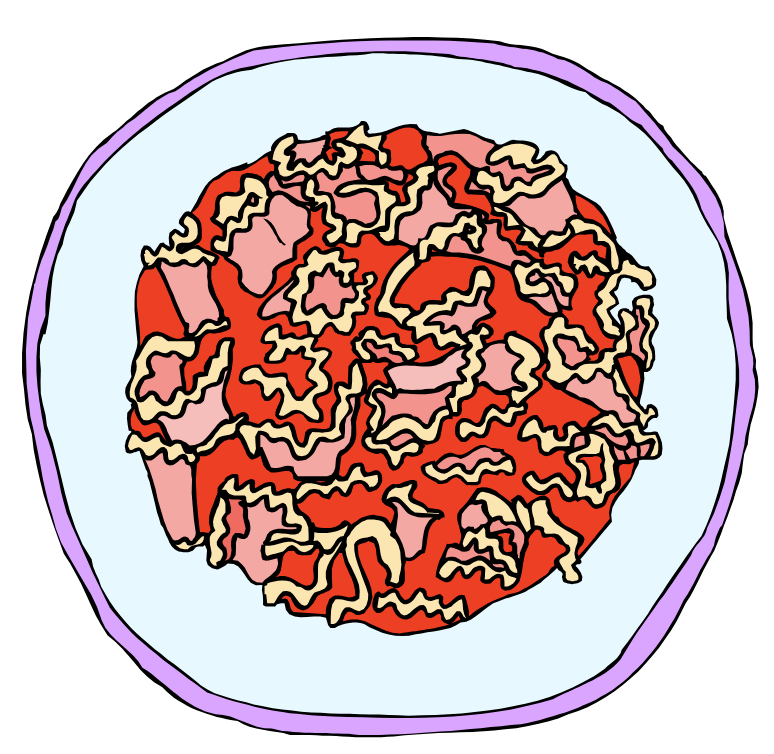
\includegraphics[width=4cm]{./photos/os_spaghetti.png}
    \end{center}
    The OS has many interleaving parts that break this abstraction.
\end{example}
\section{Theory of processes, threads and related models}
\subsection{What are processes and threads?}
In the previous section, we often talked about how the \verb|OS| was a \textit{resource manager} - but 
to what is it a manager to?
\begin{center}
    To put it simply - \verb|processes|
\end{center}

But what are processes? Consequentially, what are threads?
\begin{theory}{What is a thread?} \\
    A thread is a \verb|unit of execution|. Threads execute some portion of instructions as instructed to. Threads contain
    \begin{enumerate}
        \item Program counter
        \begin{itemize}
            \item Keeps track of which instruction the thread should execute
        \end{itemize}
        \item Registers
        \begin{itemize}
            \item Threads require some memory to execute their instructions
        \end{itemize}
        \item Stack
        \begin{itemize}
            \item Threads get their own \textit{local variables}
        \end{itemize}
        \item State
    \end{enumerate}
\end{theory}
\begin{theory}{What is a process?} \\
    A process is a \verb|unit of work|. Processes manage the information required to handle threads. Processes (in our model) do not run anything themselves. Rather
    \begin{center}
        Processes contain the necessary information to create and execute threads
    \end{center}
    Processes contain
    \begin{enumerate}
        \item Threads
        \begin{itemize}
            \item The units of execution for the process' task
        \end{itemize}
        \item Process state
        \begin{itemize}
            \item Ready, blocked or running
        \end{itemize}
        \item Address space
        \begin{itemize}
            \item What regions of memory can threads use and allocate to?
        \end{itemize}
        \item Global variables
        \begin{itemize}
            \item Shared variables between all threads
        \end{itemize}
        \item Open files
        \begin{itemize}
            \item A list of open files 
        \end{itemize}
        \item Child processes
        \begin{itemize}
            \item Processes that inherit variables and other process items, but is a distinct process
        \end{itemize}
        \item Pending alarms
        \begin{itemize}
            \item Timer-based signals from the operating system
        \end{itemize}
    \end{enumerate}
\end{theory}
\begin{aside}{The four models of threads and processes}
    \begin{enumerate}
        \item Single process, single thread
        \item Single process, multiple threads
        \item Multiple processes, single thread
        \item Multiple processes, multiple threads
    \end{enumerate}
\end{aside}
\begin{example}{When and why are processes created?}
    \begin{enumerate}
        \item System initialisation
        \begin{itemize}
            \item There are processes required to run an operating system
            \item Think about your window manager, background processes that deal with resources
        \end{itemize}
        \item Process creationg \verb|syscall|
        \item User request to create a new process
        \item Initiation of a batch job
    \end{enumerate}
\end{example}
\begin{aside}{Batch job} \\
    A batch job is a non-interactive, pre-scheduled unit of work that runs without user intervention; typically in the background.
\end{aside}
\begin{example}{What are the types of process terminations?}
    \begin{itemize}
        \item Normal exit (voluntary)
        \begin{itemize}
            \item Like at the end of the process' execution
        \end{itemize}
        \item Error exit (voluntary)
        \begin{itemize}
            \item An error occured during the unit of work - exit cleanly
        \end{itemize}
        \item Fatal error (voluntary)
        \begin{itemize}
            \item A severe runtime error that is unrecoverable, and is terminated by the \verb|OS|
        \end{itemize}
        \item Killed by another process
        \begin{itemize}
            \item For example, if a process is in deadlock or the system is out of resources
        \end{itemize}
    \end{itemize}
\end{example}
\subsection{How are processes and threads managed in an OS?}
\begin{theory}{Process Control Block (PCB)} \\
    The \verb|process control block| is a data structure that contains all of the information the OS needs to manage and execute a process (as outlined before).
    \newline \\ 
    \textbf{At the creation of a process}, a \verb|PCB| is allocated with initialisation, and is 'scheduled'.
\end{theory}
\begin{example}{How are \textit{all of} the processes stored in an OS?}
    Processes require multiple data structures to be 'stored'. There exists a \verb|process table| which stores all of the processes in the OS.
    \newline \\ 
    There also exists the \verb|ready queue| and \verb|blocked queue(s)| which relate to thread and process states.
\end{example}
\begin{theory}{Thread and process states} \\ 
    Processes, and therefore their threads have three states:
    \begin{enumerate}
        \item Running
        \item Blocked
        \item Ready
    \end{enumerate}
    \begin{center}
        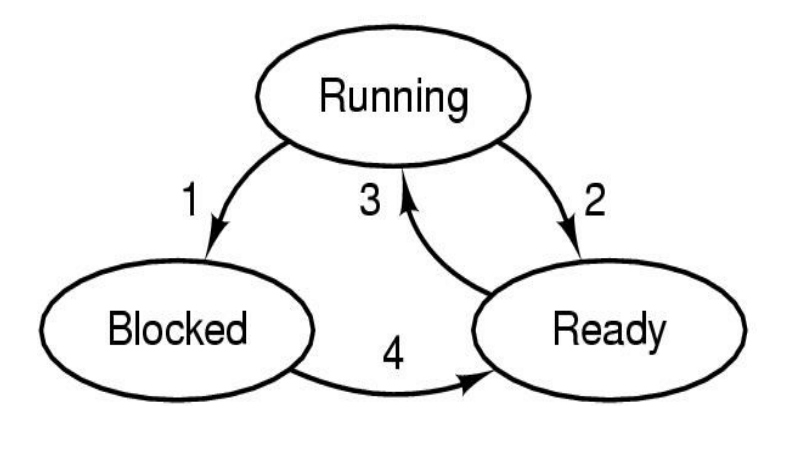
\includegraphics[width=6cm]{./photos/thread_states.png}
    \end{center}
    Consider the following actions for the above diagram
    \begin{enumerate}
        \item The running process blocks for input (\verb|I/O|)
        \item Scheduler now needs to schedule a ready process
        \item Scheduler picks a process that is ready
        \item Input event finishes, and now blocked process is ready
    \end{enumerate}
\end{theory}
\begin{aside}{The scheduler} \\
    The scheduler is an OS component which is responsible for \textbf{deciding which process or thread that runs next} on a \verb|CPU|.
\end{aside}
\begin{theory}{The ready queue} \\
    The ready queue is a queue of processes that are available to run on a CPU. The scheduler chooses from the ready queue w.r.t a pre-determined scheduling policy (for example, \verb|FCFS|)
\end{theory}
\begin{theory}{The blocked queue} \\
    When an unblocking event occurs, how do we admit this process back into the ready queue?
    \begin{itemize}
        \item Using a single blocked queue caused \verb|head-of-line| blocking
        \item This is due to the fact that not all blocks are caused by the same cause
    \end{itemize}
    Therefore, having a queue for each blocking event is the optimal (and implemented) solution
\end{theory}
\subsection{Examples of process and thread model}
\begin{example}{The hamburger restaurant - why ready/blocked queues are important} \\ 
    Imagine a hamburger restaurant - we need to grill burgers, fry the fries, prepare the burgers,
    clean the restaurant and much more. \\ \\ 
    We can imagine that we \textit{shouldn't wait for the burgers to grill}, when we could be frying the fries during this time. This is why blocking and these queues are so important.
\end{example}
\begin{example}{A diagram of a ready queue and blocked queue interaction}
    \begin{center}
        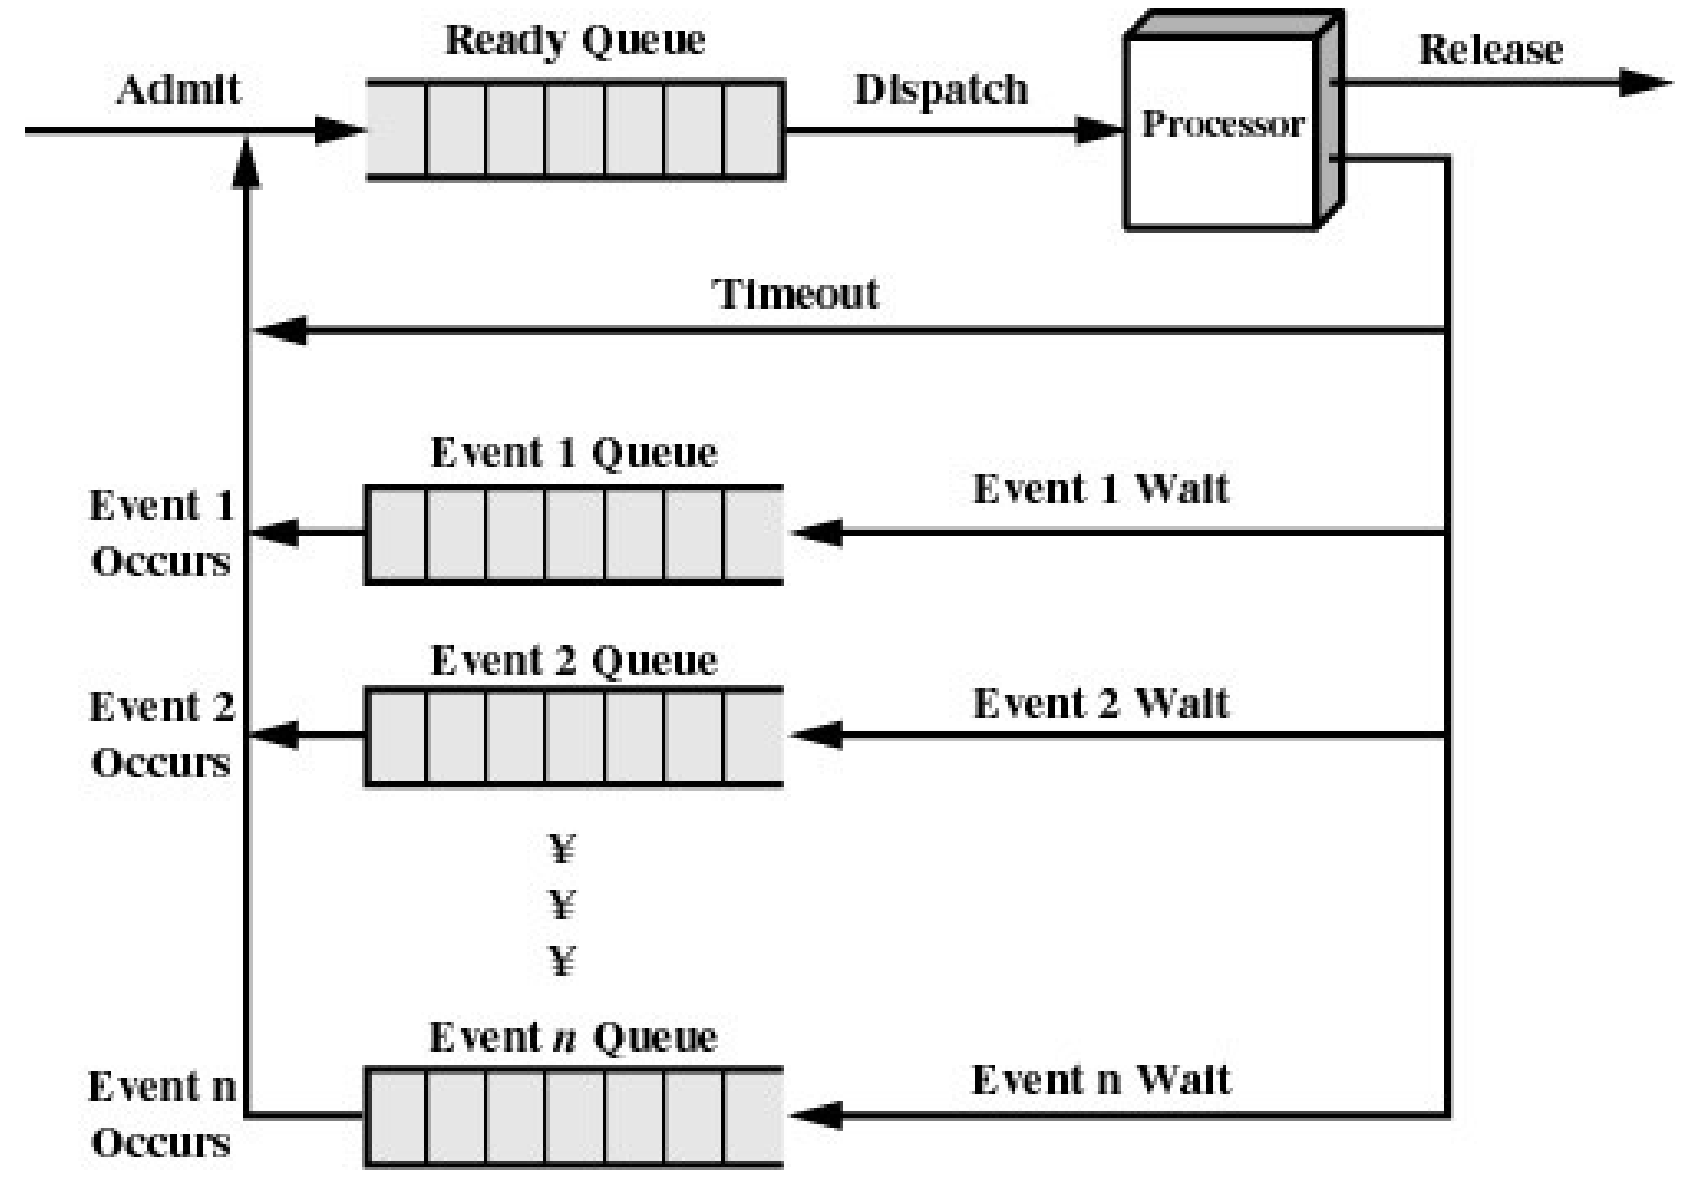
\includegraphics[width=7.5cm]{./photos/ready_blocked.png}
    \end{center}
\end{example}
\begin{aside}{Global and local variables: heap or stack?}
    \begin{itemize}
        \item Local variables are per-thread and allocated on the stack
        \item Global variables are shared across threads and alloacted in the data segment
        \item Dynamic memory can be both global or local (depending on the pointer scope)
    \end{itemize}
\end{aside}
\begin{example}{Why might multiple threads be useful? A web server example} \\ 
    Consider a web server that runs a chat function for \verb|Messenger|. Each time a user enters a chat,
    there must be some connection established.
    \begin{itemize}
        \item Imagine if we had one thread dealing with millions of different connections
        \item Users would receive messages from other users in wildly different times
        \item Rather, a per-user thread model created by a \verb|dispatcher| thread would be much more efficient
    \end{itemize}
        \begin{center}
        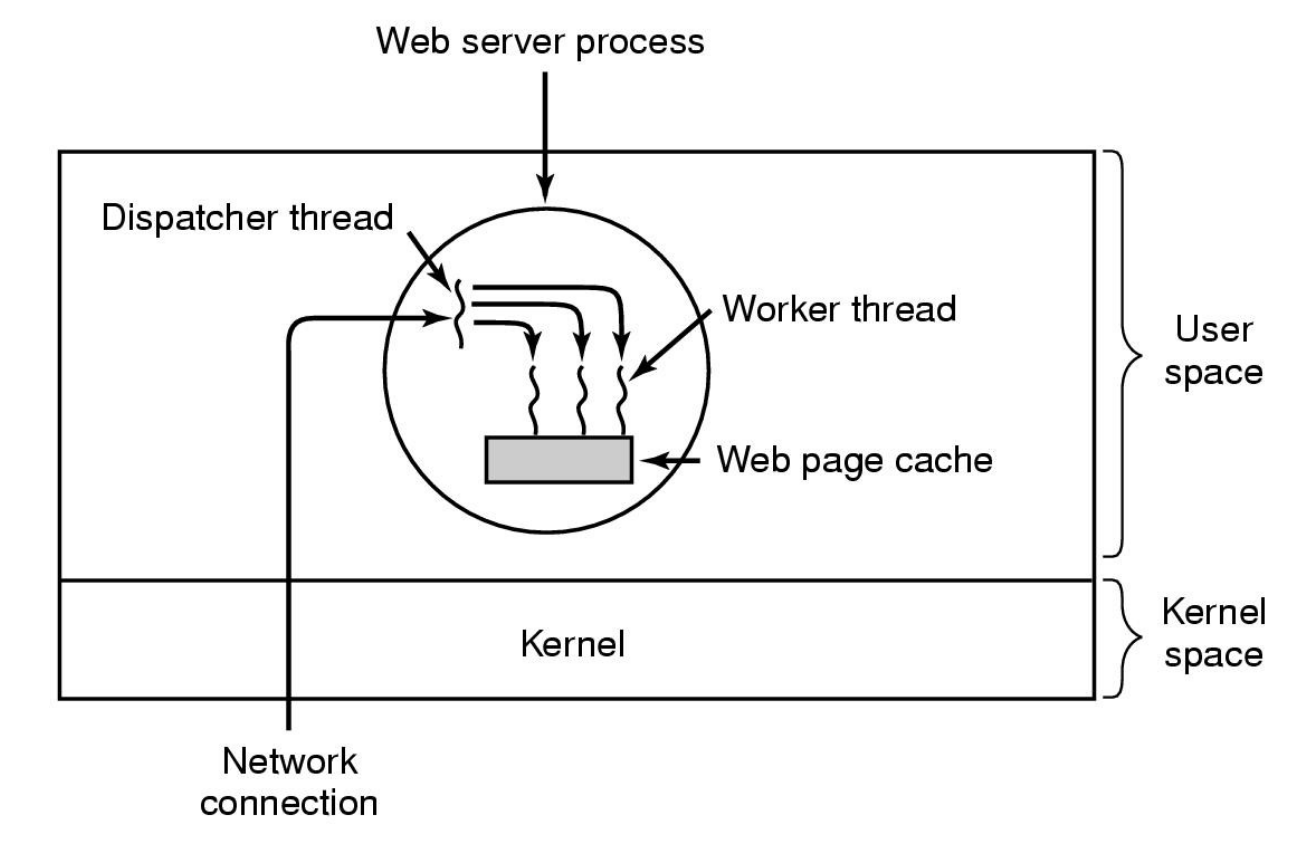
\includegraphics[width=7.5cm]{./photos/network_example.png}
    \end{center}
\end{example}
\begin{aside}{Thread model versus finite state machine} \\
    We generally think about units of execution in terms of threads - where multiple threads can concurrently run independently and in parallel.
    \newline \\
    A \textit{alternative} to this is the finite state machine (\verb|FSM|) model. In the \verb|FSM| model, systems are always in one state at a time, and transition to other states based on input. Instead of blocking, \verb|FSM|s tend to loop whilst they are waiting for an appropiate input.
\end{aside}
So why the thread model over finite state machines?
\begin{itemize}
    \item Simpler to program than a state machine - we have functions available to us from modern OSes for the implementation of processes and threads
    \item Less resources associated, and importantly resources can be shared
    \item Threads can easily take advantage of the parallelism available on machines with more than one CPU
    \begin{itemize}
        \item \verb|FSM|s run in single-threaded event loops, not ideal to take advantage of multiple processors.
    \end{itemize}
\end{itemize}
\section{Concurrency and sychronisation}
\subsection{What is concurrency and it's implications?}
With modern day compute, operating systems must be able to efficiently utilise multiple cores and parallelism capabilities.
\begin{center}
    Concurrency is when multiple tasks make progress during the same time period
\end{center}
\begin{theory}{A race condition} \\
    A race condition is when the behaviour or outcome of a program depends on the timing or ordering of events, particularly between threads.
\end{theory}
\begin{example}{A simple race condition example} \\ 
    Consider the following code 
\begin{verbatim}
void increment() {
    int t;
    t = count;
    t += 1;
    count = t;
}

void decrement() {
    int t;
    t = count;
    t -= 1;
    count = t;
}
\end{verbatim}
If two threads entered decrement and executed the instructions at the exact same time, then if the original count was \verb|1000| - both threads would result with \verb|999|.
\end{example}
\begin{aside}{But what if I use single-threaded processes!} \\ 
    While the user-level applications may be single-threaded, the kernel can interrupt at different points of the execution.
    \newline 
    Therefore, even in single threaded processes, processes that share state may still have issues with concurrency.
\end{aside}
\begin{theory}{Critical regions and their requirements} \\
    A critical region is a portion where a shared resource is accessed or modified.
    \newline \\
    The four formal requirements for a critical region are
    \begin{enumerate}
        \item Mutual exclusion: at most one thread is inside the critical region at a time 
        \item Progress: if not thread is in the critical region, and some wish to enter, one will succeed
        \item Bounded waiting: no thread should wait forever to enter the region
        \item Atomicity: the code inside a critical region appears to run atomically
    \end{enumerate}
\end{theory}
\subsection{Avoidance and detection of critical regions}
\begin{aside}{Avoiding critical regions and mutual exclusion}
    Mutual exclusion is a property of a system that ensures no two processes or threads are in their critical sections at the same time.
\end{aside}
\begin{example}{Identifying critical regions} \\
    We defined before that critical regions are when a shared resource is accessed and/or modified. Consider the below code snippet
\begin{Verbatim}[numbers=left, numbersep=2mm, frame=single]
struct node {
    int data;
    struct node *next;
}
struct node *head;

void init(void) { head = NULL; }

void insert(struct item*) {
    item->next = head;
    head = item;
}

struct node *remove(void) {
    struct node *t;
    t = head;
    if (t != NULL) {
        head = head->next;
    }
    return t;
}
\end{Verbatim}
All we have to do is consider where \verb|head| is accessed or modified. This is
\begin{itemize}
    \item Lines \verb|7|
    \item Lines \verb|10-11|
    \item Lines \verb|16-18|
\end{itemize}
\end{example}
\begin{theory}{Mutual exclusion option 1: test and set instruction} \\
    With critical regions, we have a requirement of mutual exclusion - but how do we do this? Some naive solutions include:
    \begin{itemize}
        \item Using a standard variable to signal entrance (creates another critical region)
        \item Taking turns (busy-waiting wastes resources)
        \item Disabling interrupts (wastes resources, only works in \verb|kernel|)
    \end{itemize}
    So in reality, we need some help from \textbf{hardware}. The test and set instruction (\verb|TSL|):
    \begin{itemize}
        \item Checks a value at some register \verb|$lock| and if 0, sets to 1.
        \item \textit{Guarantees these two operations happen atomically}
    \end{itemize}
\end{theory}
\subsection{Techniques for mutual exclusions and their extensions}
\begin{example}{Mutual exclusion assembly example with test-and-set} \\
    We can then utilise \verb|TSL| to ensure mutual exclusion
    \begin{Verbatim}[numbers=left, numbersep=2mm, frame=single]
critical_region:
    # some critical region code

enter_region:
    tsl $register, $lock
    jnz enter_region, $register
    jal critical_region

leave_region:
    li  $lock, 0
    ret
    \end{Verbatim}
    Here's what the code is doing:
    \begin{itemize}
        \item Line 5 loads the value of the lock into the register and tests and sets it
        \item Line 6 loops if the lock was already taking (\verb|$lock != 0|), otherwise returns to caller
        \item Line 7 otherwise enters the critical region
        \item Line 10 unlocks the lock if we have entered the region
    \end{itemize}
\end{example}
\begin{aside}{But we're still busy-waiting!} \\
    That's true! Instead of busy waiting, we could \verb|sleep| threads that attempt to enter the region but fail.
    \newline \\ 
    It is then up to the thread that is \textit{in the critical region} to wake up the next process... but which process? We will answer this question in a later mutual exclusion option.
\end{aside}
\begin{example}{The producer-consumer problem} \\
    The problem involves a \textit{producer} that creates data 
    and a \textit{consumer} that consumes data in a finite buffer.
    \begin{itemize}
        \item Consider that the buffer is finite - and so:
        \begin{itemize}
            \item the producer shouldn't produce when the buffer is full
            \item the consumer shouldn't consume when the buffer is empty
        \end{itemize}
        \item So how do we keep an accurate count?
    \end{itemize}
    We would eventually get to some stage where we lock the portion which inserts/removes items from the buffer and increments/decrements the count.
    \newline \\ 
    We are motivated to sleep when a consumer/producer can't do anything - but
    \begin{Verbatim}[numbers=left, numbersep=2mm, frame=single]
# for the producer
prod() {
    if (count == N)
        sleep(producer)

    # some code regarding the buffer

    if (count == 1)
        wakeup(con)
}

# for the consumer
con() {
    if (count == 0)
        sleep(con);

    # some code regarding the buffer

    if (count == N - 1)
        wakeup(prod);
}
    \end{Verbatim}
    We can imagine with parallel execution that we could wake up the consumer before it even sleeps, which is clearly an issue. This motivates our next data structure
\end{example}
\begin{theory}{Mutual exclusion option 2: resources and semaphores} \\
    Test and set instructions let us impose mutual exclusion on a region of code - but the producer-consumer problem showed us that with some semblance of \textit{limited resources}, we need more.
    \newline \\
    \verb|Semaphores| are a primitive that include two main instructions:
    \begin{itemize}
        \item Wait (\verb|P|): try to access the resources
        \item Signal (\verb|V|): release a resource
    \end{itemize}
    When there are multiple waiting processes, we represent this with a linked list.
    \begin{Verbatim}[numbers=left, numbersep=2mm, frame=single]
struct sempahore {
    int count;
    struct process *L;
}

P(semaphore S, process P) {
    while (S.count <= 0) {
        append P to S.L
        sleep(P)
    }
    S.count--;
}

V(sempahore S){
    S.count++;
    if (S.count <= 1) {
        fetch P from S.L
        wakeup(P)
    }
}
    \end{Verbatim}
\end{theory}
We can imagine that a \textit{critical region}, is then simply a quasi-(producer consumer) problem with 1 resource. The buffer is the region of code itself, and threads can take and reliquinish that region of code.
\begin{example}{Solving the producer-consumer problem with semaphores} \\
    \begin{Verbatim}[numbers=left, numbersep=2mm, frame=single]
#define N = 10;
semaphore mutex = 1;
sempahore buffer_empty_space = N;
sempahore buffer_filled_space = 0;

prod() {
    while (TRUE) {
        item = produce();
        wait(buffer_empty_space);
        wait(mutex);
        insert_item();
        signal(mutex);
        signal(buffer_filled_space);
    }
}

con() {
    while (TRUE) {
        wait(buffer_filled_space);
        wait(mutex);
        cons = insert_item();
        signal(mutex);
        signal(buffer_empty_space);
    }
}
    \end{Verbatim}
    We can see that
    \begin{itemize}
        \item Line 9 indicates that we will be taking some empty space from the buffer
        \item Line 13 signals to a waiting process that we have filled some space
        \item Line 19 indicates that we will be taking something from the buffer
        \item Line 23 indicates that we have taken something, and there is more empty space
    \end{itemize}
\end{example}

So, we've evolved test and set instructions $\rightarrow$ sempahores, making a higher level abstraction of 'resources' to solve our producer-consumer problem. But sempahores themselves are primitive (in the literal sense too) - they provide
two functions. Is there an easier 

\begin{theory}{Mutual exclusion option 3: easing concurrency and monitors} \\
    Monitors are a higher level programming construct which involve \textit{packaging} procedures, variables and data types into a special kind of module.
    \newline \\ 
    Importantly, only one process/thread can be in the monitor at one time, which then creates a queue-like behaviour.
    \newline \\ 
    Within the monitor, different threads may require other threads to finish to continue. In monitors, we use \verb|Condition Variables| to solve this problem.
    \begin{aside}{Condition variables}
        To allow a process to wait within the monitor, condition variables can be used.
        \newline For some condition \verb|condition x|, we can
        \begin{itemize}
            \item \verb|x.wait()|: suspended until a signal
            \item \verb|x.signal()|: resumes one suspended process.
        \end{itemize}
    \end{aside}
    \begin{center}
        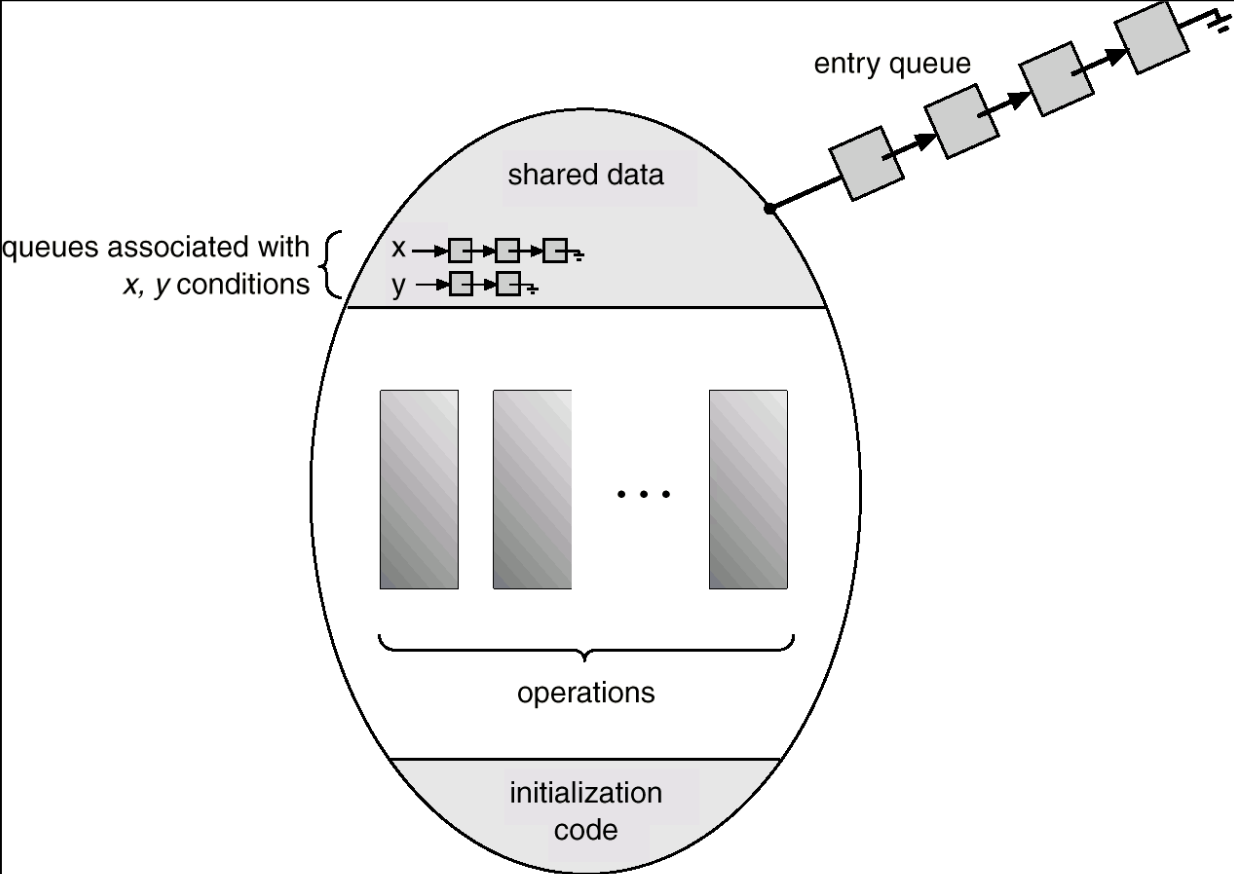
\includegraphics[width=7.5cm]{./photos/monitor.png}
    \end{center}
    \begin{center}
    Key takeaway: monitors allow for you to enter a critical region/producer-consumer problem without the worry of manually signalling semaphores or mutexes.
    \end{center}
\end{theory}
\begin{aside}{Locks, sempahores and condition variables: why, and where?} \\ 
    We've introduced these three primitives, but what purposes to they serve?
    \begin{itemize}
        \item Locks: waiting for a shared resource
        \item Semaphores: to solve the producer/consumer problem
        \item Condition variables: waiting for an event
    \end{itemize}
\end{aside}
\begin{example}{The dining philosophers problem} \\
    To conclude our chapter in concurrency and synchronisation, we look to the dining philosophers problem. Five philosophers can either eat or think about eating.
    \begin{center}
        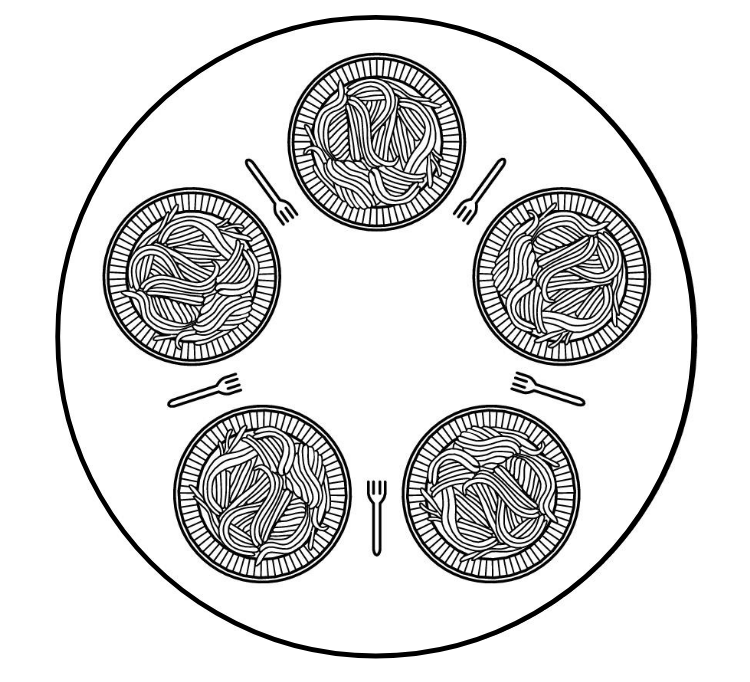
\includegraphics[width=6cm]{./photos/dining_philosophers.png}
    \end{center}
    The philosophers can only pick up one fork at a time. How do we solve this problem?
    \begin{Verbatim}[numbers=left, numbersep=2mm, frame=single]
monitor DiningPhilosophers {
condition can_eat[5];
state[5] = THINKING;

procedure pickup(i) {
    state[i] = HUNGRY;
    test(i);
    if (state[i] != EATING) 
        wait(can_eat[i]);
}
procedure putdown(i) {
    state[i] = THINKING;
    test((i+4)%5);  # left
    test((i+1)%5);  # right
}
procedure test(i) {
    if (state[i] == HUNGRY &&
        state[(i+4)%5] != EATING &&
        state[(i+1)%5] != EATING) {
        state[i] = EATING;
        signal(can_eat[i]);
    }
}
}
    \end{Verbatim}
\end{example}
\begin{aside}{Heuristically identifying deadlocks} \\
    To maintain safe concurrent interactions, there must be a \textit{global locking order}. That is, if some process $A$ locks in the order $L_1 \to L_2 \to L_3$, then every other process which also utilises these locks must lock in this order.
    \newline \\ To find deadlock conditions, we consider the lock order of each process, and find any inversions of the global locking order.
\end{aside}
\section{MIPS R3000, and practical implementation of processes and threads}
I assume you remember most of the instructions for MIPS from COMP1521. I mention some interesting implementation details about MIPS R3000, and as well include register conventions.
\subsection{MIPS details}
\begin{aside}{MIPS pipelining and the branch delay slot}
    \begin{center}
        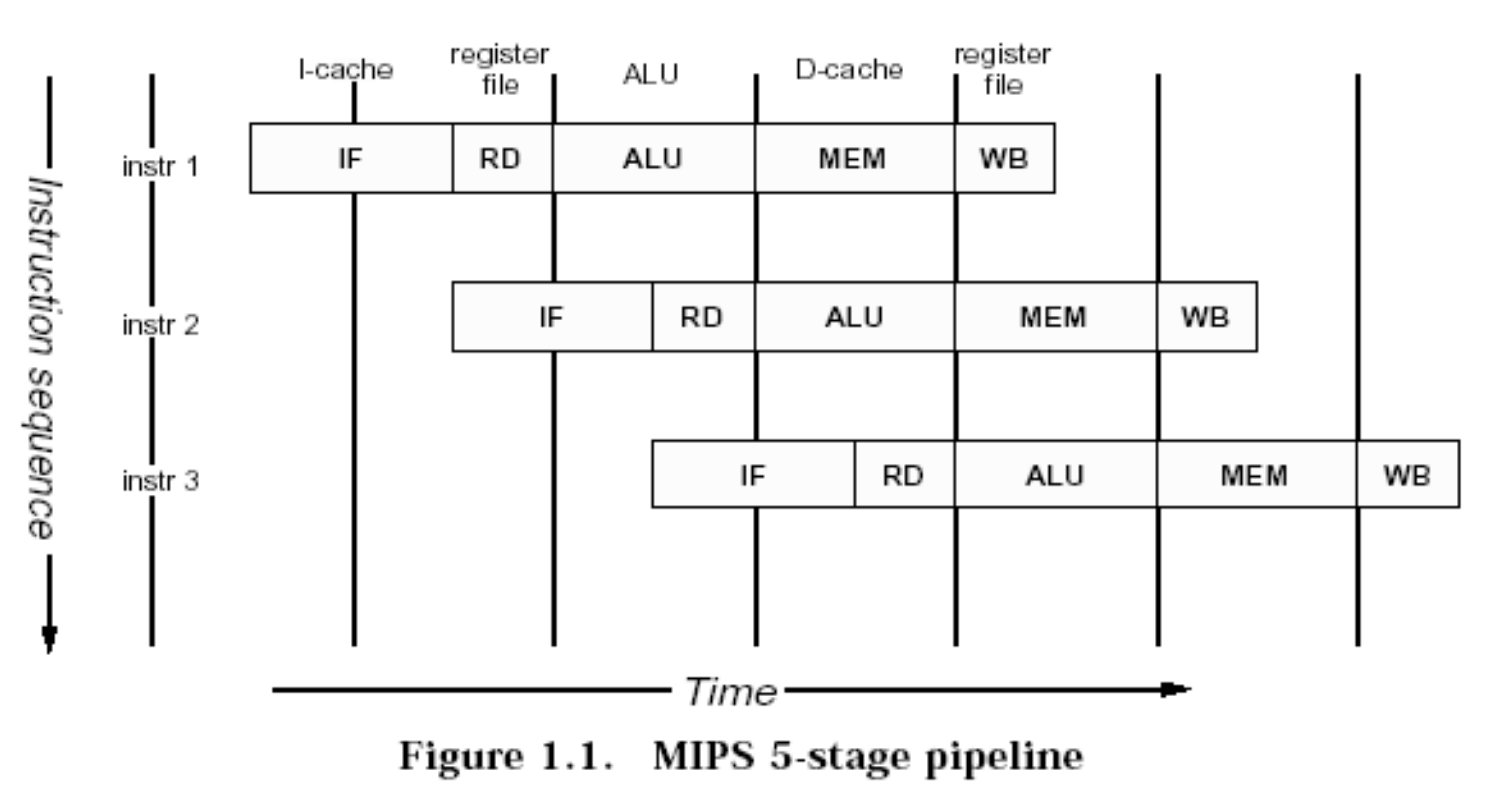
\includegraphics[width=7.5cm]{./photos/mips_pipeline.png}
    \end{center}
    MIPS R3000 pipelines it's instructions for efficiency. We can see in the above diagram that there are three instructions being pipelined. 
    \newline \\ 
    The \verb|branch decision| is not known until the end of the \verb|ALU| phase - so if instruction 2 relies on instruction 1, then it must wait until the end of instruction 1's \verb|ALU| phase.
    \newline \\
    \textit{This is why there exists a branch delay} for MIPS R300 jump instructions. For example
    \begin{Verbatim}[numbers=left, numbersep=2mm, frame=single]
jal 1f
nop     # nothing occurs here
lw r4, (r6)
    \end{Verbatim}
    After the jump on line 1, the jump only takes place on the third line \textit{before} it is executed. Once it returns, it will continue on line 3.
\end{aside}
\begin{aside}{The program counter (PC)} \\ 
    The program counter is used to keep track of which instruction to run next. In \verb|MIPS R3000|, instructions are \verb|32-bits|, and thus \verb|4| bytes. 
    \newline \\ 
    Thus, after a (non-jump) instruction, the PC increments 4 bytes
    \begin{center}
        \verb|PC += PC + 4|
    \end{center}
    For a jump instruction, the program counter jumps the PC to the location, and then jumps back 
    and then starts at 8 bytes forward of the jump (due to the branch delay).
\end{aside}
\newpage
\begin{aside}{Compiler register conventions}
    \begin{center}
        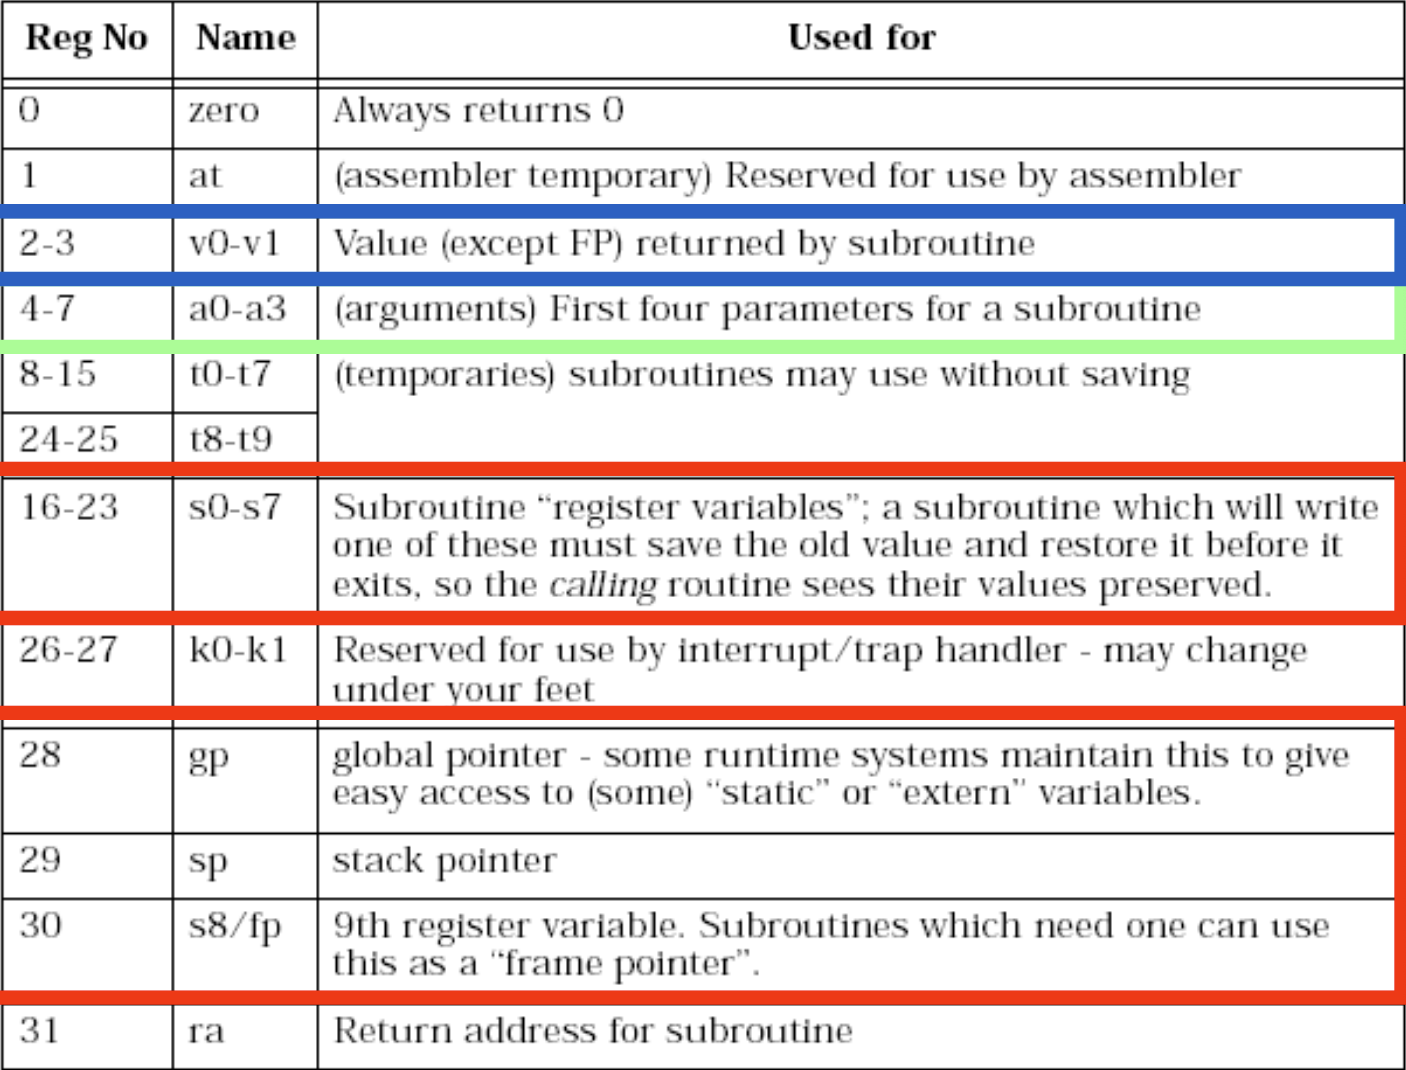
\includegraphics[width=7.5cm]{./photos/compiler_register_conventions.png}
    \end{center}
\end{aside}
\begin{theory}{Per-thread stack components: stack frames} \\
    Previously, we mentioned how threads have their own per-thread stack. \textit{Similarly}, functions have their own per-function \verb|stack frame|, which stores:
    \begin{itemize}
        \item The return address for the function
        \item Saved registers
        \item Passed function parameters
        \item Local varaibles
    \end{itemize}
    \begin{center}
        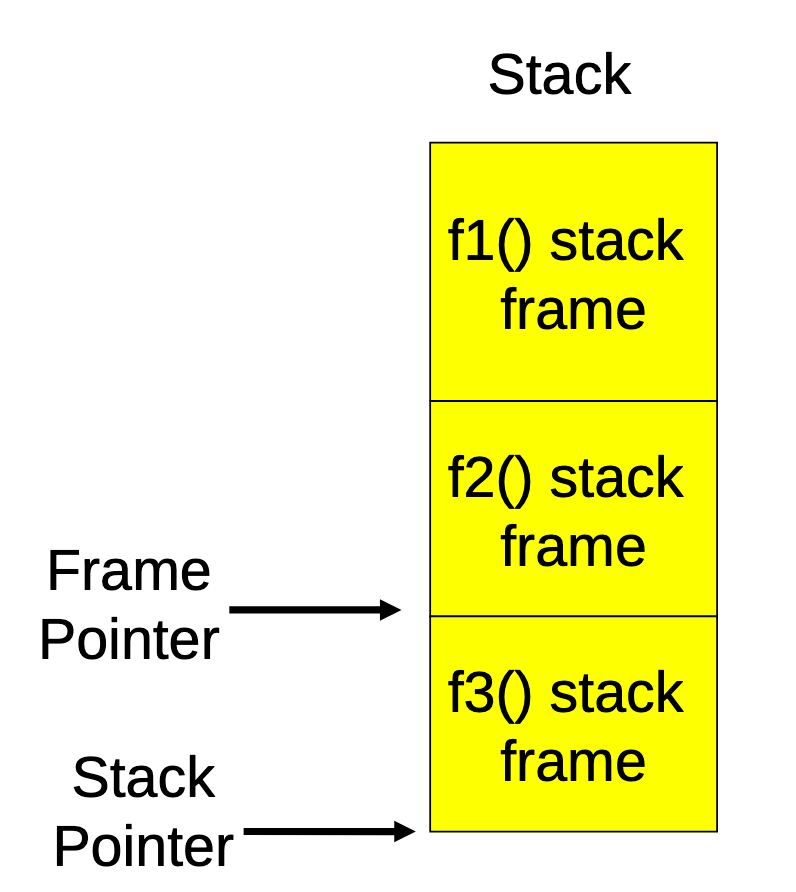
\includegraphics[width=5cm]{./photos/stack_frame.png}
    \end{center}
    The stack grows downwards, and winds up as functions return (this is not strictly true and can be seen in the reverse way).
\end{theory}
\begin{aside}{So how do we know where to go back to after a jump?} \\
    Using stack frames! The stack frame stores the appropiate return address (program counter) for the function. When we do
    \begin{verbatim}
0x00: jal function_one
    \end{verbatim}
    We are creating a new stack frame for the function \verb|function_one|, with information including that the return address is \verb|0x00 + 4|.
\end{aside}
Okay, so we now know how per-thread stack space's are divvied up (using stack frames). What about processes?
\begin{theory}{Process memory layout} \\
    We consider a single-threaded process below. \\ \\
    Remember that the process contains everything a unit of work requires to run. At the minimum, the contains three segments:
    \begin{enumerate}
        \item Text
        \begin{itemize}
            \item Contains the code (instructions) to run
        \end{itemize}
        \item Data
        \begin{itemize}
            \item Global variables
        \end{itemize}
        \item Stack
        \begin{itemize}
            \item Activation records of procedures/function/method
            \item Local variables
        \end{itemize}
    \end{enumerate}
    \begin{center}
        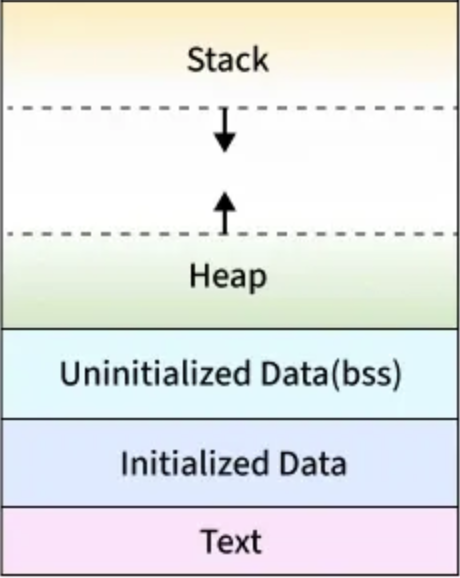
\includegraphics[width=6cm]{./photos/process_memory.png}
    \end{center}
\end{theory}
Processes exist in both user and kernel mode, so how do they differ?
\begin{theory}{Processes in user and kernel mode} \\
    User processes
    \begin{itemize}
        \item User processes are scheduled by the kernel
        \item They are isolated from eachother
        \item The OS ensures no concurrency issues exist
    \end{itemize}
    Kernel processes
    \begin{itemize}
        \item Mostly the same as user processes, but\dots
        \item Kernel memory is shared between all processes
        \item Concurrency issues can exist with system calls
    \end{itemize}
\end{theory}
Now let's talk about threads - should they be instantiated at the user or kernel level? 
\begin{theory}{User-level versus kernel-level threads} \\
    User-level threads
    \begin{itemize}
        \item Processes create threads without the knowledge of the OS, so\dots
        \item Have to deal with concurrency issues, \verb|yield| within process
        \item Can create many more threads
        \item Does \textit{not} take advantage of multiple CPUs
        \item If a thread blocks, the entire process blocks (wasting \verb|I/O| time!)
    \end{itemize}
    Kernel-level threads
    \begin{itemize}
        \item Preemption - threads cannot hog CPU indefinitely
        \item True parallelism, overlap blocking \verb|I/O| with CPU-bound
        \item But creation/destruction requires kernel entry/exit, which is expensive
    \end{itemize}
\end{theory}
\begin{aside}{Cooperative versus preemptive multithreading} \\
    User-level threads are not within the kernels control, and thus are not subject to the scheduler. This means that
    any form of multi-threading must be \textit{cooperative} - that is, must be voluntary \verb|yielded|.
    \newline \\ 
    Kernel-level threads are controlled by the kernel, and are thus preemptively multithreaded; they can be paused mid execution by the scheduler.
\end{aside}

So both user and kernel level threads have their own advantages and disadvantages. For these notes, we generally assume kernel-level threads.
\newline \\ 
We have talked about the idea of \textit{switching} between processes, as well as threads within processes. What's
happening here?
\subsection{Context switching: implementation and implications in the kernel}
\begin{theory}{Context switch} \\
    A context switch can refer to both:
    \begin{itemize}
        \item a switch between threads
        \item a switch between processes
    \end{itemize}
    It is easy to wonder how we can switch back and forth, consider the per-thread/per-process memory we are required to have.
    \newline \\ 
    A switch can occur any time we enter the kernel, so
    \begin{enumerate}
        \item on a \verb|syscall|
        \item on an exception
        \item on an interrupt
    \end{enumerate}
\end{theory}
\begin{theory}{Trapframe} \\
    A trapframe is a snapshot in time of the CPU's state. It is used in context switches to 
    save the state of execution for a thread/process.
    \newline \\
    They are often represented in \verb|struct|s with the registers as variables.
\end{theory}

\begin{aside}{Thread switching: what occurs?} \\
    Let us walk through what occurs during a thread switch, from thread \verb|T1 -> T2|.
    \begin{enumerate}
        \item We begin with the stack pointer pointing to T1's stack \verb|$sp$|
        \item After an exception/syscall/interrupt, we switch to the kernel stack
        \item We push T1's trapframe onto the kernel stack.
        \item We call some \verb|C| code that processes the exception/syscall/interrupt
        \item The kernel decides to context siwtch - we then push the kernel state onto the stack
        \item We switch to another process, which then unwinds down from the above process
    \end{enumerate}
    \begin{center}
        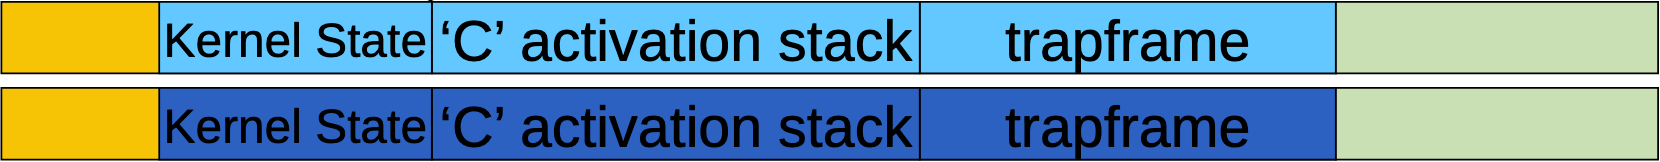
\includegraphics[width=7.5cm]{./photos/thread_switch.png}
    \end{center}
\end{aside}
\begin{example}{What's in the kernel state?} \\
    In the kernel state, a few important (and some still unlearned data structures) exist
    \begin{itemize}
        \item Page tables (for virtual memory mapping)
        \item Kernel stack pointer (to know where to unwind from)
        \item Scheduling information
        \item Locks, resourecs, etc.
    \end{itemize}
\end{example}
\section{System calls}
\begin{center}
    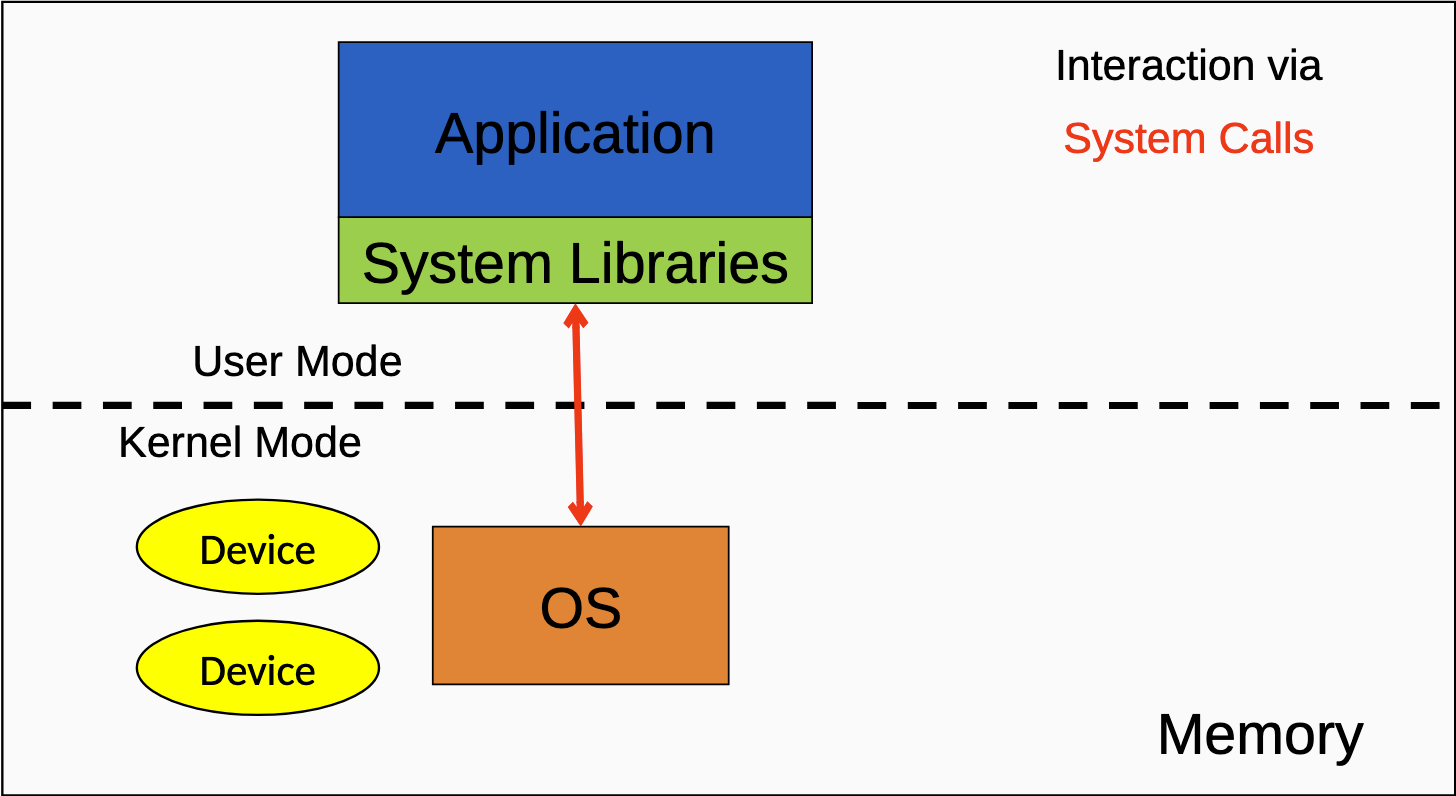
\includegraphics[width=7.5cm]{./photos/syscall_system.png}
\end{center}
We have previously referred to \verb|syscall|s, as ways to enter the kernel (the OS) and access privilieged operations. In this section, we consider what actually occurs during a syscall.

\begin{theory}{Some important registers for syscalls}
    \begin{center}
        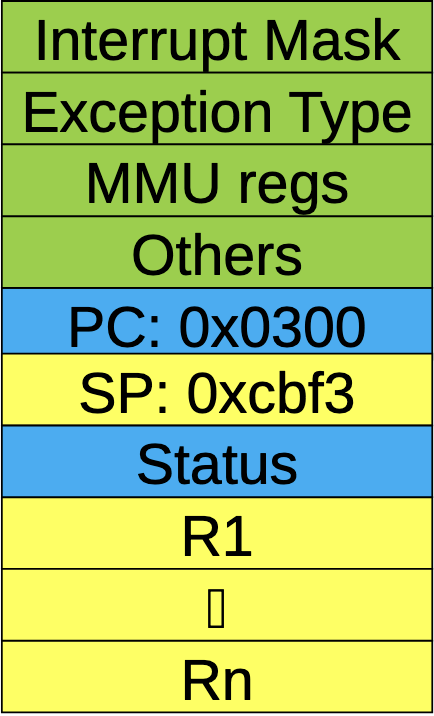
\includegraphics[width=3.5cm]{./photos/registers.png}
    \end{center}
    Some of the above registers are important for understanding system calls.
    \begin{itemize}
        \item Interrupt mask: a bitmask that determines which interrupts are enabled/disabled.
        \item Exception type: indicates what caused the trap (kernel entry), for e.g system call, page fault, etc
        \item MMU (Memory Management Unit) regs: stores info about the process' memory mapping
        \item PC: Program Counter
        \item SP: Stack Pointer
        \item Status: Contains information about condition codes, privilege codes and interrupt enable bits
    \end{itemize}
\end{theory}
\begin{aside}{Privilieged portions of memory} \\ 
    There exists memory addresses that are only accessible to the kernel. The exact ranges are usually configurable.
    \begin{itemize}
        \item This is done to protect kernel code and data
    \end{itemize}
\end{aside}
Before we begin explaining how system calls are entered, processed and then exited, we must first consider some software/hardware details regarding MIPS R3000.
\begin{theory}{Coprocessor 0 (CP0)} \\ 
    The processor control registers are located in CP0. These registers control
    \begin{itemize}
        \item Exception/interrupt management registers
        \item Translation management registers
    \end{itemize}
    Specific instructions are used to manipulate CP0, and are \textit{only accessible in kernel mode}. There are 3 important registers we would like to focus on:
    \begin{itemize}
        \item \verb|c0_cause|: cause of the recent exception
        \item \verb|c0_status|: current status of the CPU
        \item \verb|c0_epc|: address of the instruction that caused the exception
    \end{itemize}
    What information do these registers contain?
    \begin{aside}{c0\_status}
        \begin{itemize}
            \item \verb|IM|: 8 bits of interrupt mask bits. 6 external, 2 software.
            \item \verb|KU|: user or kernel mode? \verb|0| is kernel, \verb|1| is user
            \item \verb|IE|: \verb|0| is all interrupts masked, \verb|1| is interrupts enabled
            \item \verb|c, p, o|: current, previous, old which exists for \verb|KU| and \verb|IE|
        \end{itemize}
    \end{aside}
    \begin{aside}{c0\_cause} 
        \begin{itemize}
            \item \verb|ExcCode|: the code number of the exception taken
        \end{itemize}
        Each exception code has a mapping to a specfiic reasoning. The two important ones to know are \verb|0| for interrupt and \verb|8| for syscall.
    \end{aside}
    \begin{aside}{c0\_epc}
        This register points to the address of where to \textit{restart} execution after handling the exception.
    \end{aside}
    \begin{aside}{Exception vectors}
        Exception vectors are fixed memory addresses which the processor jumps to for specific exceptions.
        \newline \\ 
        This means there's no need for dispatching - thus no need for \verb|c0_cause|. The exception code used for general exceptions is \verb|0x80000080|.
    \end{aside}
\end{theory}
\begin{example}{Full walkthrough of an hardware exception handler} \\
    We begin with
\begin{verbatim}
PC: 0x12345678  | EPC: ?
Cause: ?        | Status: ?|?|?|?|1|1
\end{verbatim}
where status is \verb|KUo,IEo,KU,IEp,KUc,IEc|. An interrupt exception occurs at the current
program counter.
\begin{verbatim}
PC: 0x12345678  | EPC: 0x12345678
Cause: 0        | Status: ?|?|1|1|0|0 
\end{verbatim}
Note the cause \verb|0| which corresponds to interrupt. Also note that the current \verb|KU, IE| have been shifted downwards to the previous flags.
\begin{verbatim}
PC: 0x80000080  | EPC: 0x12345678
Cause: 0        | Status: ?|?|1|1|0|0 
\end{verbatim}
We now place the program counter to the general exception vector placed in PC. Now we know what caused the exception, and where to restart once we deal with it. Let us assume the exception is dealt with,
and has the following variable states
\begin{verbatim}
PC: 0x80001234  | EPC: 0x12345678
Cause: 0        | Status: ?|?|1|1|0|0 
\end{verbatim}
Now consider the following assembly code to return to program
    \begin{Verbatim}[numbers=left, numbersep=2mm, frame=single]
lw r27, saved_epc
nop
jr r27
rfe
    \end{Verbatim}
    Line 1 stores the address where the exception occured back into the PC. We then do a \verb|rfe| instruction, which is a \verb|return from exception| instruction.
\begin{verbatim}
PC: 0x12345678  | EPC: 0x12345678
Cause: 0        | Status: ?|?|?|?|1|1 
\end{verbatim}
And we are now back at the user-level, executing our program from where an interrupt was raised.
\end{example}
\begin{theory}{MIPS and OS/161 Syscall Conventions} \\
    MIPS
    \begin{itemize}
        \item Syscalls are invoked by the \verb|syscall| instruction
        \item Syscalls are represented by numbers, and must be agreed on by convention with the caller.
        \item A convention is required as to how user-level software indicates
        \begin{itemize}
            \item Which system call is required
            \item Where it's arguments are
            \item Where the result should go
        \end{itemize}
    \end{itemize}
    OS/161
    \begin{itemize}
        \item Arguments are passed and returned via the normal C function calling convention, i.e \verb|def read_syscall(int fd)|
        \item Syscalls are defined by a syscall \textbf{number} - agreed on convention
        \item Register \verb|v0| contains the syscall number
        \item On return, \verb|a3| contains:
        \begin{itemize}
            \item 0 for success, and \verb|v0| contains the result
            \item not 0 for failure, and \verb|v0| has the error number
        \end{itemize}
    \end{itemize}
\end{theory}
\begin{aside}{What occurs on the user side of the syscall?}
    \begin{itemize}
        \item The user side is pretty straight forward
        \item Call the desired \verb|syscall| with the correct arguments
    \end{itemize}
\end{aside}
\begin{aside}{What occurs on the kernel side of the syscall?}
    \begin{itemize}
        \item Change to kernel stack
        \item Preserve registers by saving to kernel stack
        \item Leave saved registers somewhere accessible
        \item Complete the \verb|syscall|
        \item Restore registers
        \item Switch back to the user stack
        \item Return to application
    \end{itemize}
\end{aside}
\begin{example}{What occurs in a computer during an exception that causes a context switch?} \\
    Consider an interrupt on a thread causes a thread switch. Detail what occurs throughout
    the user and kernel level.
    \begin{enumerate}
        \item CPU: some interrupt is raised, and an exception is generated
        \item CPU: changes to kernel mode and calls the exception handler at \verb|0x8000080|
        \item Exception handler: switches to the kernel stack pointer
        \item Exception handler: saves the user registers for the interrupt process to the stack
        \item Exception handler: determines the source of the interrupt - let's say it was a \verb|timer| interrupt, and switches to the timer interrupt handler.
        \item Timer interrupt handler: acknowledges the interrupt, and calls the scheduler
        \item Scheduler: chooses a new process to run, and then invokes the kernel to switch
        \item Kernel: saves the current stacks kernel context to the kernel stack
        \item Kernel: switches to the new thread's stack by moving \verb|$sp|
        \item Kernel: reads the new process in-kernel context from the stack
        \item Kernel: restores the user registers for the new process
        \item Kernel: set the processor back to user mode
        \item Kernel: jump to new user process' PC
    \end{enumerate}
    Note where different portions of the original thread state is saved (user + kernel state)
\end{example}
\begin{aside}{MIPS R3000 does not have specific exception handlers!} \\ 
    Besides for specifc exceptions (e.g \verb|TLB| misses in a specific memory region), MIPS forwards all exceptions to the general exception vector \verb|0x80000080|.
    \newline \\
    \textit{From there}, different specific handlers/routines can be called, after the handler figures out the specific exception that occured.
\end{aside}
\section{Deadlocks and Livelocks}
We have talked to a decent extent about \verb|resources| and how to avoid problems with shared resources between multiple threads/processes. In this seciton, we talk about the problem of deadlocks and livelocks - where progress cannot be made due to a resource.
\begin{theory}{What is a resource?} \\
    Formally, a resource is a physical \textit{or logical/digital} entity required for process execution, that is controlled by the \verb|OS|.
\end{theory}
\begin{theory}{What is a deadlock?} \\
    A deadlock is a state of a system in whcih a finite set of processes are waiting for an event that can only be caused by another process in the same set.
    \begin{itemize}
        \item Suppose process $P_1$ holds resource $A$ and requests resource $B$
        \item Suppose process $P_2$ holds resource $B$ and requests resource $A$
    \end{itemize}
    Clearly there is no progress that can be made here.
\end{theory}
This should motivate some formal requirement regarding the \textit{ordering} of how resources are taken.
\begin{aside}{The four conditions for a deadlock}
    \begin{enumerate}
        \item Mutual exclusion
        \begin{itemize}
            \item Each resource is either assigned to a process or is available
        \end{itemize}
        \item Hold and wait condition
        \begin{itemize}
            \item A process which already has resources can request more resources
        \end{itemize}
        \item No preemption condition
        \begin{itemize}
            \item Resources granted to other processes cannot be forcibly taken away
        \end{itemize}
        \item Circular wait condition
        \begin{itemize}
            \item Must be a circular chain of requests of 2 or more processes
        \end{itemize}
    \end{enumerate}
\end{aside}
We can very quickly, heuristically argue why these conditions are required
\begin{enumerate}
    \item If a resource was infinite, then no deadlocks could possibly occur
    \item If a process could only hold one resource, then it would never depend on another resource held by another process
    \item If a process could be preempted, then a deadlocked process could just take it
    \item There is a requirement for $A -> B$ and $B -> A$ for no progress to be made (consider a circular path)
\end{enumerate}
\begin{example}{Representing deadlocks} \\
    Deadlocks are often represented by directed graphs, with the tail at the resource and the head at the process.
    \begin{center}
        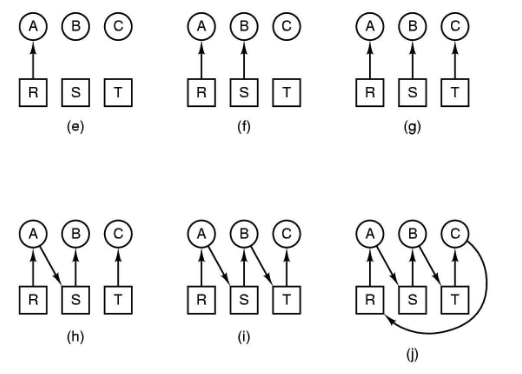
\includegraphics[width=7cm]{./photos/deadlock.png}
    \end{center}
    Here $\{R, S, T\}$ are resources and $\{A, B, C\}$ are resources.
\end{example}
The four broad approaches for dealing with deadlocks is
\begin{enumerate}
    \item Just ignore the problem
    \item Prevent the problem (negate one of the conditions)
    \item Detection and recovery
    \item Dynamic avoidance (careful resource allocation)
\end{enumerate}
\begin{theory}{Approach 1: The Ostrich Algorithm} \\
    The first approach is to do nothing - this is reasonable only if
    \begin{enumerate}
        \item deadlocks occur very rarely
        \item cost of prevention is high
    \end{enumerate}
    This is a tradeoff between \verb|convenience| and \verb|correctness|.
\end{theory}
\begin{theory}{Approach 2: Deadlock Prevention} \\
    In deadlock prevention, we aim to negate one of the four conditions of a deadlock. Consider how we could do this for each condition:
    \begin{aside}{Mutual exclusion}
        \begin{itemize}
            \item Not feasible - requires finite resources to become infinite
            \item If we removed locks, then concurrency issues
        \end{itemize}
    \end{aside}
    \begin{aside}{Hold and wait}
        \begin{itemize}
            \item Requires processes to request all resources before starting
            \item This is of course difficult to know at runtime
            \item We \textit{could} make a process give up all resources if it is required to block holding a resource, but this could cause \verb|livelock| (explained after).
        \end{itemize}
    \end{aside}
    \begin{aside}{No preemption}
        \begin{itemize}
            \item Not feasible to take away a resource from a process mid execution
            \item Hard to identify what resources are crucial to a process, etc.
        \end{itemize}
    \end{aside}
    \begin{aside}{Circular wait}
        \begin{itemize}
            \item We could attack this by carefully ordering resources
        \end{itemize}
    \end{aside}
\end{theory}
\begin{aside}{What is a live lock?} \\
    Livelocked processes are not blocked, change state regularly but never make progress.
    \newline \\
    Imagine two resources constantly releasing and re-requesting a lock, but ordering makes it so that neither of the two processes can enter the critical region.
\end{aside}
\begin{theory}{Approach 3: Detection and Recovery} \\
    Assuming a system is deadlocked, we require a method to detect this and restore progress.
    \newline \\ 
    Consider the following graph model. We have processes $P = \{P_1, \dots, P_n\}$ and resources $R = \{R_1, \dots, R_k\}$. The \verb|OS| then holds a resource allocation graph (RAG)of
    \begin{align}
        P_i &\to R_j: \text{ request edge} \\
        R_j &\to P_i: \text{ assignment edge}
    \end{align}
    If there exists any cycles, then there is a deadlock. For multiple-instance resources,  this doesn't necessarily mean there is a deadlock. We need
    \begin{itemize}
        \item \verb|avail|: a $k \times 1$ vector of free instances of resources $R_j$
        \item \verb|alloc|: a $n \times k$ matrix where \verb|alloc[i][j]| is instances of $R_j$ held by $P_i$
        \item \verb|req|: a $n \times k$ matrix where \verb|req[i][j]| is instances of $R_j$ that $P_i$ still needs to finish
    \end{itemize}
    We therefore have the algorithm
{\small
\begin{Verbatim}[numbers=left, numbersep=2mm, frame=single]
finish = false for n x 1

repeat
    found = false
    for i from 1 to n
        if !finish && req <= work:
            avail[i] = avail[i] 
                     + alloc[i]
            finish[i] = true
            found = true
        end if
    end for
until found = false

deadlock = [
    f for i in finish where i is false
]
\end{Verbatim}
}
\begin{itemize}
    \item Line 6 considers whether there is enough resources to fulfill the request
    \item If there is, line 7 completes that request, and then restores the freed resources
    \item If any process finishes without being found, then they are deadlocked.
\end{itemize}
\end{theory}
\begin{aside}{But how do we recover?} \\
    We generally recover by simply killing one or more processes of the deadlocked transaction.
\end{aside}
\begin{theory}{Approach 4: Deadlock Avoidance} \\
    Deadlock avoidance is possible, but we need to know \textit{the maximum number of each resource required} by each process. There are two main ways we can represent this
\begin{center}
    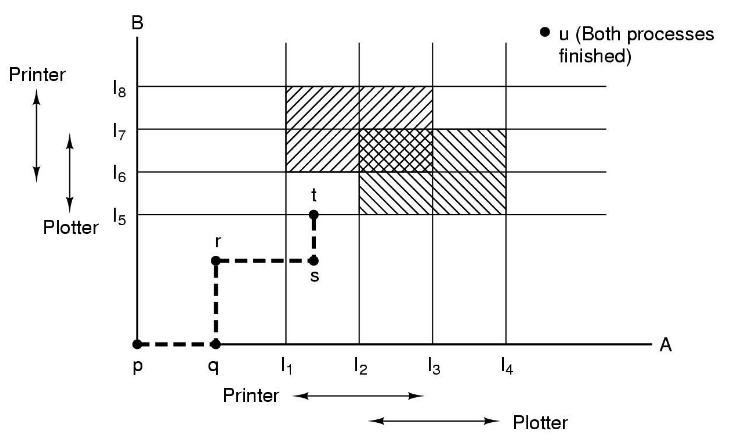
\includegraphics[width=7.5cm]{./photos/resource_trajectories.png}
    \captionof*{Fig}{Resource trajectories}
\end{center}
    \begin{itemize}
        \item In the above figure, we see a resource trajectory graph of two process $A$ and $B$
        \item Consider the regions $I_1 \to I_4$ for $A$ and $I_6 \to I_8$ for B.
        \item Both require the printer, and so $t$ has entered an unsafe state 
    \end{itemize}
\begin{center}
    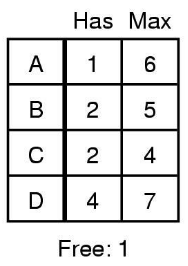
\includegraphics[width=3.5cm]{./photos/bankers_algo.png}
    \captionof*{Fig}{Banker's algorithm}
\end{center}
\begin{itemize}
    \item Instead consider we are given a table of resources, with processes $A, B, C, D$
    \item The \verb|Has| column is the currently held resources, the \verb|Max| is the max number of resources
    \item \verb|Free| denotes the number of free resources available in the system
    \item In this case, we should not allocate any more resources, otherwise the system is in an unsafe state (zero resources)
    \item This is called the \textit{Banker's Algorithm}
\end{itemize}
\end{theory}
\begin{aside}{What is starvation?} \\
    In the first section of the course, we discovered that an operating system should ensure that starvation does not occur.
    \newline \\ 
    Starvation is when a process \textit{never receives} the resource it is waiting for, despite the resource repeatedly becoming free.
    \begin{itemize}
        \item This may be due to an inappropiate or inefficient allocation algorithm
    \end{itemize}
\end{aside}
\section{File management and file systems}
We discuss file systems and virtual file systems in the context of \verb|UNIX| systems. Before this, we consider conventions about files and dircetories and what must be decided by the file system.
\subsection{File system components}
\begin{example}{File names}
    \begin{itemize}
        \item Textual names, which may have restrictions
        \begin{itemize}
            \item Only certain characters
            \item Limited length
            \item Certain format
        \end{itemize}
        \item Can be case sensitive
        \item Names may obey inventions (e.g \verb|.c| for C files)
    \end{itemize}
\end{example}
\begin{example}{File structure (or the absence of)}
    \begin{itemize}
        \item Files are generally just a sequence of bytes
        \item \textit{Most} OS have unstructured files
        \item Structured files may have advantages in efficiency (the OS knows where things are before hand), but are hard to port to other OS.
    \end{itemize}
\end{example}
\begin{example}{File types}
    \begin{itemize}
        \item Regular files, directories, device files, streams/pipes
    \end{itemize}
\end{example}
\begin{example}{File access types}
    \begin{enumerate}
        \item Sequential access 
        \begin{itemize}
            \item Linearly scan the file from the \verb|0|-th position
            \item No jumping around (no \verb|SEEK_SET|)
        \end{itemize}
        \item Random access
        \begin{itemize}
            \item Can be read in any order
            \item The read can be one of two options
            \begin{enumerate}
                \item Move file pointer (\verb|seek|) and then read, or
                \item Each read specifies the file pointer
            \end{enumerate}
        \end{itemize}
    \end{enumerate}
\end{example}
\begin{aside}{Giving the OS context in unstructured files: Executable Link Format} \\
    Through a \textbf{Executable Linkable Format (ELF)}, the OS is informed of the location of important components. If the file is an executable, for example
    \begin{itemize}
        \item Provides information about the file; 32-bit vs 64-bit, endiannes, entry point address
        \item How parts of the file should be mapped into virtual memory
        \begin{itemize}
            \item \verb|text|, \verb|data|, \verb|stack|, \verb|heap|
        \end{itemize}
        \item Context for the linker
    \end{itemize}
\end{aside}
\begin{example}{File directories} 
    \begin{itemize}
        \item Provides mapping between the file names and the file (data) themselves
        \item Contains informations about files
        \begin{itemize}
            \item attributes, location, ownership and more
        \end{itemize}
        \item Directories themselves are specially structured files owned by the OS
    \end{itemize}
\end{example}
\begin{aside}{Tracking the current working directory + relative path names} \\
    Constantly using the absolute path name is tedious, and so the current working director (\verb|cwd|) \verb|./| is convenient. We can also do \textit{relative} paths - for example \verb|../| indicating the parent directory of the \verb|cwd|.
\end{aside}
\begin{example}{Access rights and simultaneous access rights}
    \begin{itemize}
        \item We might want some users to be able to read, but not write
        \item Might not want some users to be able to delete
        \item Access rights come with the following operations
        \begin{itemize}
            \item \verb|execution|, \verb|reading|, \verb|appending|
            \item \verb|updating|, \verb|rights change|, \verb|deletion|
        \end{itemize}
        \item The \verb|owner| as all rights
    \end{itemize}
    One might wonder how the \verb|OS| deals with simultaneous access to files. Typically one of two approaches
    \begin{enumerate}
        \item User may lock entire when when updated, or
        \item User may lock individual records/ranges of the file while updating
    \end{enumerate}
\end{example}
That is (most) all of the file semantics/properties we care about when we wish to implement a file system. We now consider the implementation of file systems in a UNIX-like system.
\vspace{-1em}
\subsection{UNIX File Systems and Components}

\begin{theory}{The UNIX Storage Stack: explained}
    \begin{gather*}
    \text{Application} \\
    \downarrow \\
    \text{FD table} \\
    \downarrow \\ 
    \text{OF table} \\ 
    \downarrow \\ 
    \text{Virtual file system} \\
    \downarrow \\
    \text{File system(s)}\\
    \downarrow \\
    \text{Buffer cache} \\ 
    \downarrow \\
    \text{Disk scheduler} \\
    \downarrow \\
    \text{Device driver} \\
    \downarrow \\
    \text{Disk controller + disk}
    \end{gather*}
    We will explain the stack bottom up
    \begin{itemize}
        \item The disk controller handles disk geometry and exposes the disk as a linear sequence of 'blocks'
        \item The device driver abstracts device specific (so disk, solid state, etc) protocol. Also exposes the linear sequence of blocks
        \item The file system abstracts the linear sequence of blocks into a directory hierarchy
        \item The buffer cache sits between the file system and disk scheduler for performance, keeping \textit{recently accessed disk blocks}
        \item The virtual file system aggregates multiple file systems to be one interactable file system across multiple devices
        \item The open file table is a global table of all the open files on a system
        \item The file descriptor table is a per-process table of the files open in a process
        \item The application interacts with files through \textit{file descriptors}.
    \end{itemize}
\end{theory}
\begin{aside}{Locality and speed: getting close} \\
    Many file systems are designed for spinning disks - the mechanism of a spinning disk works by reading disks as they spin.
    \\ \\
    Consider sequentially reading some file subdivided into blocks $F = \{F_1, F_2, ..., F_b\}$. We can imagine that as
    $$ ||F_{i+1} - F_i|| \to \infty$$
    where, reading the file becomes very slow (imagine a file evenly spread out across the entire revolution).
    \begin{center}
        Blocks being close together (locality) is important for read speed
    \end{center}
\end{aside}
So how should blocks be allocated? If we use disks, should we just allocate them sequentially? We explore the following methods of 'block' allocation:
\begin{enumerate}
    \item Contiguous allocation (sequential)
    \item Dynamic allocation 
    \begin{itemize}
        \item Blocks as linked lists
        \item File allocation table
        \item Index nodes (\verb|inode|)
    \end{itemize}
\end{enumerate}
\begin{aside}{What is a 'block'?} \\
    Blocks are \verb|fixed| (but generally configurable) partitions of disk space. Data is split up into 'blocks' when written to disk.
\end{aside}
\begin{aside}{What happens when you delete a block in a file system?} \\
    When you 'delete' a block, the block simply gets marked as writeable. The block itself does not get zeroed out, so it does not require an additional \verb|I/O| operation.
\end{aside}
\begin{theory}{Contiguous allocation}
    \begin{center}
        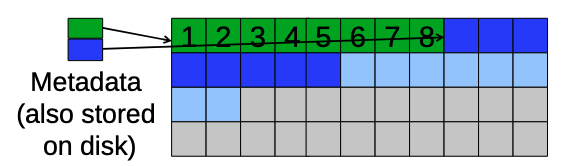
\includegraphics[width=7.5cm]{./photos/contig_alloc.png}
    \end{center}
    Write the file to disk in sequential blocks.
    \begin{itemize}
        \item[\ding{51}] Easy bookkeeping (starting block + length)
        \item[\ding{51}] $\uparrow$ performance for sequential operations
        \item[\ding{55}] External fragmentation
        \item[\ding{55}] As files are deleted, free space becomes divided into small (mostly unusable) space
    \end{itemize}
\end{theory}
\begin{aside}{Fragmenting our disk: externally and internally}
    External fragmentation is
    \begin{itemize}
        \item space wasted externally to allocated memory regions
        \item memory may exist, but is not contiguous (and thus cannot be written for contiguous alloc)
    \end{itemize}
    Internal fragmentation is
    \begin{itemize}
        \item space wasted internally to allocated memory regions
        \item for example, block sizes are too large and are thus not utilised appropiately
    \end{itemize}
\end{aside}
\begin{theory}{Dynamic allocation: linked list allocation}
    \begin{center}
        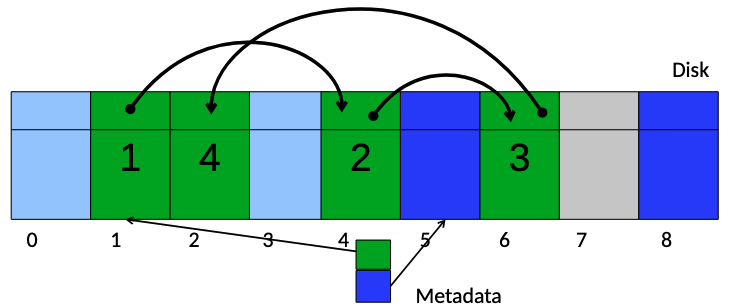
\includegraphics[width=7.5cm]{./photos/linked_list_alloc.png}
    \end{center}
    We place blocks whether there is space, and represent the ordering of files in a linked list. The block number of the next block is stored in each block.
    \begin{itemize}
        \item[\ding{51}] One single metadata entry per file (starting block number, etc)
        \item[\ding{51}] Best for sequentially accessed files
        \item[\ding{55}] Bad for random access (we have to linearly scan!)
        \item[\ding{55}] Blocks are scattered across the disk  
    \end{itemize}
\end{theory}
\begin{theory}{Dynamic allocation: File Allocation Table (FAT)}

    We keep a $1:1$ copy of the file system (linked list alloc) in a separate table in memory.
    \begin{itemize}
        \item[\ding{51}] Random access is faster, as in-memory scan is fast.
        \item[\ding{55}] Memory usage becomes big, fast. 
    \end{itemize}
    \verb|200 GB| is \verb|200 * 10^6 * 10^3| bytes. With \verb|1K| byte blocks, we have \verb|200 * 10^6| blocks. This means there are \verb|200 * 10^6| FAT entries in RAM, which means it takes up
    $$ \verb|800 MB|$$
    which is substantial.
\end{theory}
\begin{aside}{What happens if something corrupts or we lose the table in memory?} \\
    For \verb|FAT| implementations, there exists redundancies stored on disk to be pulled into memory in case any corruption occurs.
    \begin{center}
        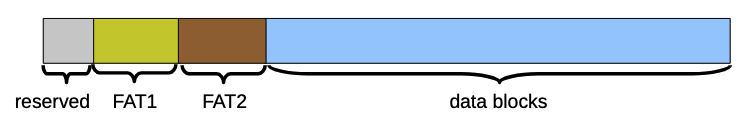
\includegraphics[width=7.5cm]{./photos/fat_redundancy.png}
    \end{center}
\end{aside}
\begin{theory}{Dynamic allocation: inode-based}
    \begin{center}
        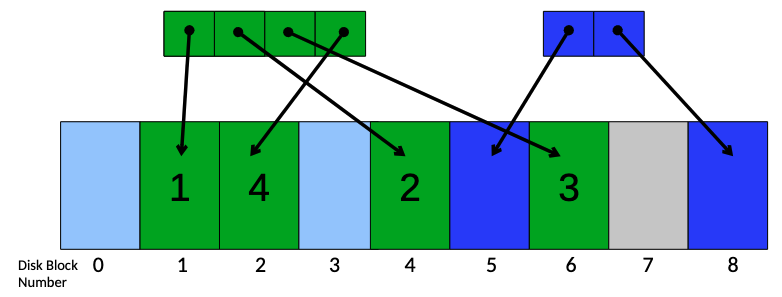
\includegraphics[width=7.5cm]{./photos/inode_alloc.png}
    \end{center}
    The key idea is to keep a separate table (called a \verb|inode|) for each file.
    \begin{itemize}
        \item Only keep table for open files in memory (borrowing ideas from \verb|FAT|)
        \item So we get fast random acess
    \end{itemize}
    \verb|inodes| are allocated dynamically, and free-space management is required for inodes. Inode's keep pointers to addresses of disk blocks, and then an indirection pointer to another block of pointers.
    \begin{center}
        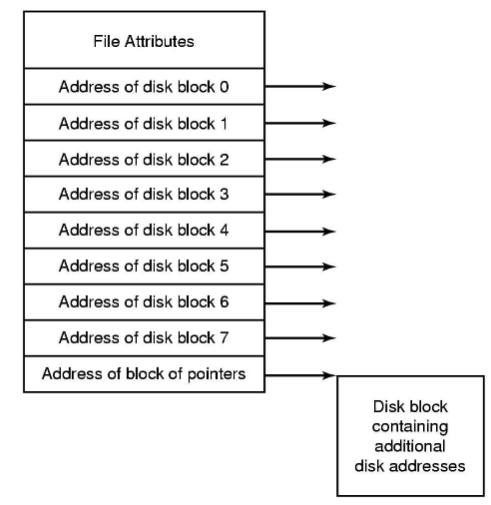
\includegraphics[width=7.5cm]{./photos/inode_blocks.png}
        \captionof*{Fig}{Blocks + an indirection blocks}
    \end{center}
\end{theory}
\begin{example}{Comparing the three methods for different situations} \\
    Consider a file with 100 records. Compare how many \verb|I/O| operations are required for contiguous allocation, linked allocation and indexed (direct pointer) allocation compares with the following 6 scenarios
    \begin{enumerate}
        \item The record is added at the beginning
        \item The record is added in the middle
        \item The record is added at the end
        \item The record is removed from the beginning
        \item The record is removed from the middle
        \item The record is removed from the end
    \end{enumerate}
    \begin{center}
        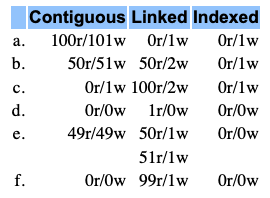
\includegraphics[width=6.5cm]{./photos/alloc_comp.png}
    \end{center}
    Note for indexed allocation, that deletes just requires an update in memory noting that the block is writeable/free.
    \newline \\ 
    For linked list, we need to write the new block but also update the previous blocks "next pointer", so we require 2 writes for some scenarios.
\end{example}
\begin{aside}{Implementing inodes: keeping track of free space} \\
    So how do we keep track of these blocks, and how do we manage free space? There are two approaches
    \begin{enumerate}
        \item Linked list of free blocks in free blocks on disk
        \item Bitmaps of free blocks and free i-nodes on disk
    \end{enumerate}
    \begin{aside}{Free block list} One free block creates a linked list to information about other free blocks
        \begin{itemize}
            \item List of all unallocated blocks
            \item Store within the fre blocks themselves
            \item Only one block of pointers need to be kept in main memory
        \end{itemize}
    \end{aside}
    \begin{aside}{Bitmap} Individual bits in a bit vector represent used/free blocks.
        \begin{itemize}
            \item One bit represents one block
            \item Expensive to search
            \item Easy to find contiguous free space (consecutive \verb|0|s)
        \end{itemize}
    \end{aside}
\end{aside}
\begin{theory}{Implementation of directories} 
    \begin{itemize}
        \item Directories are stored like normal files, inside data blocks
        \item File systems assign special meanings to the content of these files
        \begin{itemize}
            \item A directory file is a \textit{list} of directory entries
            \item A directory entry contains a file name, attributes and the file \verb|inode| number
        \end{itemize}
    \end{itemize}
    The \verb|inode| number can then be used to access the file's contents.
\end{theory}
\begin{aside}{So how do we choose what block size to use?}
    \begin{itemize}
        \item Larger blocks require less meta data but incur more internal fragmentation
        \item Smaller blocks incur less internal fragmentation
        \item Larger blocks are better for sequential operations, less \verb|I/O|
        \item But for random access, smaller blocks load less unrelated data
    \end{itemize}
    So block size is a compromise, and is dependent on the requirements of the machine.
\end{aside}
So we know how file systems are implemented (generally for \verb|disks|), but how do \textit{virtual} file systems combine them to create a single unified abstraction for file usage?
\begin{theory}{Providing a unified abstraction: vnodes/VFS} 
    There are two major components to a virtual file system. The \verb|vfs|, which represents all file systems:
    \begin{itemize}
        \item Contain pointers to functions to do file-system-wide operations (e.g unmount, mount)
    \end{itemize}
    \verb|vnodes|, represent a file (\verb|inode|) in an underlying (abstracted) file system.
    \begin{itemize}
        \item Contains pointers to functions to manipulate files/inodes (e.g open, close, etc.)
    \end{itemize}
    \begin{center}
        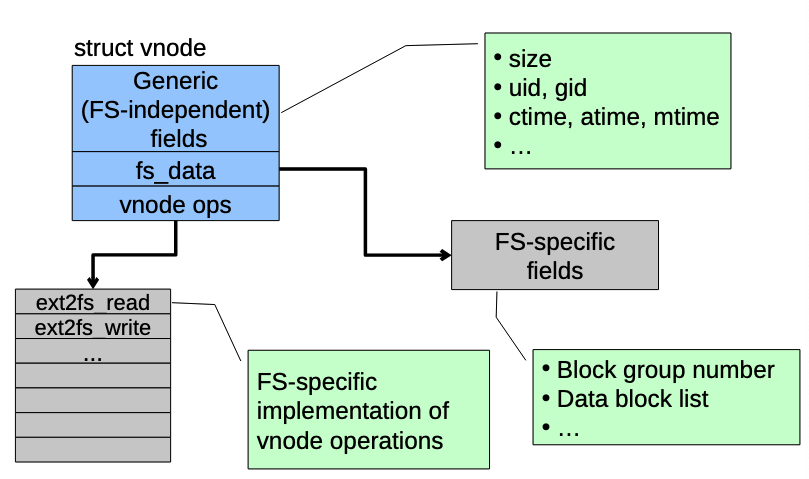
\includegraphics[width=7.5cm]{./photos/vnode.png}
        \captionof*{Fig}{vnode representation}
    \end{center}
    \begin{center}
        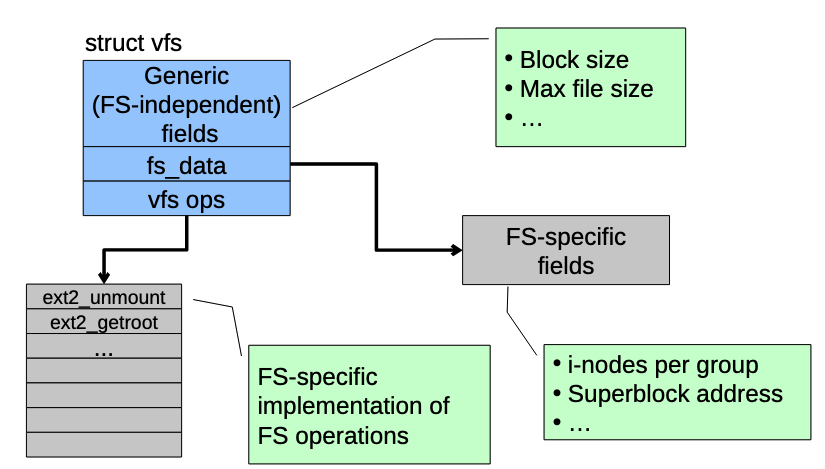
\includegraphics[width=7.5cm]{./photos/vfs.png}
        \captionof*{Fig}{vfs representation}
    \end{center}
\end{theory}
So we abstract file systems with virtual file systems. Now how do applications interact with files?
\begin{theory}{File descriptor tables and file descriptors} \\
    File descriptors (\verb|fd|) are indexes into file descriptor tables. File desriptor tables are (sometimes not literally) a table of pointers to vnodes, along with more information.
    \begin{verbatim}
struct fd {
    off_t offset;
    int readable;
    int writeable;
    int executable;
    struct vnode *v;
}
    \end{verbatim}
    Therefore when a file is opened in an application, a new file descriptor is created in it's per-process file descriptor table (which is also stored in the global open file table).
\end{theory}
\begin{aside}{What file descriptor tables are necessary?} \\
    At the very minimum, there needs to be a \textit{per-process} file descriptor
    \begin{itemize}
        \item When files are opened by two different processes, the reading/seeking/writing/etc. of one process shouldn't necessarily effect another file.
    \end{itemize}
    But some system calls like \verb|fork| require two processes to share a file pointer. So we also need a \textit{global open file table}
    \begin{itemize}
        \item This is used to point to one reference of a file descriptor from two different processes.
    \end{itemize}
\end{aside}
So now we know how applications deal with virtual file systems, how virtual file systems aggregate file systems and how file systems abstract a block sequence. How do we make these operations fast?
\begin{theory}{Buffers and caches} \\
    Buffer:
    \begin{itemize}
        \item Temporary storage used when transferring data between two entities
        \item Useful when entities transfer at different rates (e.g memory bus versus disk)
    \end{itemize}
    Cache:
    \begin{itemize}
        \item Fast storage used to temporarily hold data to speed up repeated access to data
    \end{itemize}
\end{theory}
\begin{aside}{How do file systems utilise buffers and caches?}
    Buffers
    \begin{itemize}
        \item Writes to disk can become very slow if we write directly to disk, as the speed of memory and the speed of disk is not in sync
        \item Rather, we write to a \textit{buffer}, which is then heuristically flushed to disk
        \item We can also read blocks into the buffer ahead-of-schedule to increase efficiency
    \end{itemize}
    Caches
    \begin{itemize}
        \item We often access repeated segments of data
        \item When we read segments of data, we cache them in a finite, small memory set
    \end{itemize}
    Of course, buffers and caches are related (and often integrated). There is no point of reading a block into a buffer, and separately reading it into a cache.
\end{aside}
\begin{example}{But are buffer caches an all-around win? Write-through caches} \\
    No, not necessarily. While buffer caches are important to deal with memory/disk speed discrepancies and improve read performance, for portable storage devices and other scenarios, buffers present the risk for \textbf{data to be lost}. \\ \\
    Therefore, implementing a write-through cache which write immediately can be utilised for certain devices at the sake of performance.
\end{example}
\begin{aside}{Which cached blocks should survive? Which should we discard?} 
    \begin{itemize}
        \item Since cache space is finite, we need to make decisions on what to remove.
        \item Generally prioritised in terms of system criticality - directory blocks and inode blocks are crucial
        \item Data blocks will corrupt only the file that they are associated with
        \item So remove low-priority blocks first
    \end{itemize}
\end{aside}
\subsection{Practical implementation of \texttt{inodes} and file system components}
We now look to \verb|ext2| and \verb|ext3| filesystems to explore specific components of \verb|inodes| and others to gain a better grasp of what is happening.
\begin{theory}{\texttt{ext2 file system}: indirection pointers} \\
    We previous discussed that \verb|inodes| have direct block pointers, which hold direct disk block numbers. 
    \begin{itemize}
        \item \verb|ext2| has 12 direct blocks
        \item If there are more blocks then 12, what occurs?
    \end{itemize}
    \verb|ext2| also has three indirect pointers; single, double and triple.
    \begin{enumerate}
        \item Single indirect points to a block which contains direct blocks (2 reads)
        \item Double indirect points to a block with blocks which contains direct blocks (3 reads)
        \item Triple indirect points to a block with blocks with blocks which contain direct blocks (4 reads)
    \end{enumerate}
\end{theory}
\begin{aside}{How many blocks can each indirect hold?} \\
    Assume $1$K-byte blocks, with $4$-byte block numbers.
    \begin{itemize}
        \item The single indirect contains $256$ blocks.
        \item The double indirect contains $256^2$ blocks.
        \item The triple indirect contains $256^3$ blocks.
    \end{itemize}
    So in total in \texttt{ext2}, we have a total of $256 + 256^2 + 256^3 = 16843020$ blocks, which is approximately $16$ GB
\end{aside}
\begin{example}{Where is the block number in the tree?} \\
    Assume $4$K blocks, $4$ byte block numbers and 12 direct blocks. Consider the following code excerpt
    \begin{verbatim}
lseek(fd, 1048576, SEEK_SET)
write(fd, "x", 1)
lseek(fd, 5242880, SEEK_SET)
write(fd, "x", 1)\end{verbatim}
    Find the block number of the $1048576$-th byte, and the $5242880$-th byte.
    \newline \\
    First consider the tree of blocks. We have:
    \begin{itemize}
        \item \verb|0 - 11| for direct blocks
        \item $4096 / 4 = 1024$ blocks in single indirect, so \verb|12 - 1035|
        \item $1024^2 = 1048576$ blocks in double indirect, so \verb|1036 - 1049611| 
        \item We won't need the triple indirect
    \end{itemize}
    The $1048756$-th byte is block $1048756 / 4096 = 256$. Therefore, it is in the single indirect. Specifically, it is the $256 - 12 = 244$-th block in the single indirect.
    \newline \\ 
    The $5242880$-th byte is block $5242880 / 4096 = 1280$, therefore it is in the double indirect. Specifically, it is the $1280 - 1036 = 244$-th block of the double indirect.
\end{example}
You may be wondering where \verb|inodes| are stored. While this is discretionary to the file-system, there are some considerations to be made.
\begin{aside}{Storing inodes and file system attributes: the Berkeley Fast File System (FSS)} \\
    There are four main components to the disk:
    \begin{itemize}
        \item Boot block: containing code to bootstrap the OS
        \item Super block: containing attributes of the FS (size, number of inodes, etc)
        \item Inode array: array of inodes
        \item Data blocks
    \end{itemize}
    If we stored these linearly, then we would have long seek times (seek to inode, then seek to data block), as well as redundancy issues (superblock is lost = catastrophic for FS). 
    \newline \\
    The \textit{Berkeley Fast Filesystem (FSS)} accounts for this by
    \begin{itemize}
        \item Partitioning the disc into multiple block groups
        \item Each block group has:
        \begin{itemize}
            \item A copy of the super block
            \item A copy of group descriptors
            \item Data block bitmap
            \item Inode bitmap
            \item Inode table
            \item Data blocks
        \end{itemize}
    \end{itemize}
    Group descriptors tell us:
    \begin{itemize}
        \item Location of bitmaps, counter for free blocks and inodes, number of directories in the group
    \end{itemize}
\end{aside}
We now turn to consider the implications of multiple processes interacting with file systems, and requirements of \verb|consistency| across these processes.
\subsection{File system consistency with journalling}
Systems crash and are unreliable; when crashes occur, it is imperative that once the system has recovered, that processes within the system have a reliable, universal view of the file system.
\begin{example}{When deleting a file, what steps does a UNIX system take? Why journalling is important.} \\
    When deleting a file, a UNIX file system takes the following steps
    \begin{enumerate}
        \item Mark disk blocks as free
        \item Remove the directory entry
        \item Mark the i-node as free
    \end{enumerate}
    Therefore, if there is a problem in between one of these steps, the file system may have an inconsistent state.
\end{example}
\begin{theory}{Journalling} \\
    Journalling involves writing to a buffer of sorts, which is used as a reference/record in case a crash occurs.
    \newline \\ 
    Journal entries involvefile system operations - and if changes were not flushed to disk, the OS is still able to understand what changes occured through journal entries.
\end{theory}
\begin{aside}{\texttt{ext3 filesystem:} transactions} \\ 
    Transactions in the verb|ext3| FS have four steps:
    \begin{gather*}
        \text{In Progress} \\
        \downarrow \\
        \text{Completed} \\
        \downarrow \\
        \text{Committed} \\
        \downarrow \\
        \text{Checkpointed}
    \end{gather*}
    The steps entail:
    \begin{itemize}
        \item In progress: FS updates are still buffered in RAM 
        \item Completed: Updates are buffered in ram - no additional updates for this transaction
        \item Committed: Updates are written to the journal and marked as 'committed'. This transaction can now be 'replayed'
        \item Checkpointed: Updates are written to the file system, and the transaction is removed from the journal
    \end{itemize}
\end{aside}

The \verb|Journaling Block Device (JBD)| sits in between the file system and the block device/journal, and ensures file systems transactions occur with the above steps in mind.

\section{Memory hierarchy, caching and performance}

We have talked at length across all of our sections about the requirement for performance with respect to file systems, processes/threads and more. We now consider performance with respect to memory sources, and caching performance improvements.
\begin{theory}{Memory hierarchy: speed $\uparrow$, costs $\uparrow$!}
    \begin{gather*}
        \text{Registers} \\ 
        \downarrow \\
        \text{Cache} \\
        \downarrow \\
        \text{Main memory} \\
        \downarrow \\
        \text{Magnetic disk} \\
        \downarrow \\
        \text{Magnetic tape}
    \end{gather*}
    As we descend in the above memory hierarchy, we incur:
    \begin{itemize}
        \item Decreasing costs per bit
        \item Increasing capacity
        \item Increasing access time
    \end{itemize}
    This means that we cannot have super fast access with large capacity - memory has a tradeoff.
\end{theory}

To compensate for slower access times as we descend in the memory hiearchy, \textit{caching} is utilised all across hardware and the operating system to create performant operations.
\begin{theory}{CPU Cache} \\
    We have previously talked about what caching is. The CPU cache (\verb|SRAM|) sits between the CPU and main memory (\verb|DRAM|), and aims to reduce memory latency from CPU calls to memory.
    \begin{gather}
        \text{CPU} \\
        \updownarrow \\
        \text{CPU Cache/\texttt{SRAM}} \\
        \updownarrow \\
        \text{Main memory/\texttt{DRAM}}
    \end{gather}
    The CPU cache holds recently used data and instructions to save memory access.
\end{theory}
\begin{aside}{But how much do caches actually speed up operation?} \\
    This entirely depends on the \textit{hitrate} of the cache - how often it is utilised. Given $H$, the hitrate of the cache, $T_C$ the time to retrieve from cache and $T_M$ the time to retrive from memory, we have
    $$ T_{\text{effective}} = H \cdot T_C + (1 - H) \cdot T_M$$
    where it is assumed that $T_C < T_M$.
\end{aside}
\begin{example}{What are some other examples of cache? Spinning disks are slow!} \\
    While the \verb|CPU Cache| is in itself a cache for main memory, main memory is too a cache for hard drives/spinning disks!
\end{example}

\section{Memory management}
In memory management, we aim to answer to main concerns:
\begin{enumerate}
    \item Parititioning memory given processes are smaller than memory
    \item Partitioning memory given processes are larger than memory
\end{enumerate}
\subsection{Simpler partitioning methods, and their components}
\begin{aside}{Splitting up memory between processes: the challenge} \\
    Processes have differing requirements for memory, and also change their 
    requirements for memory dynamically.
    \newline \\
    We consider 2 broad strategies for partitioning memory for processes:
    \begin{enumerate}
        \item Fixed partitioning (equal sized, variable sized)
        \item Dynamic partitioning
    \end{enumerate}
\end{aside}
\begin{theory}{Fixed partitioning for process memory} \\
    Fixed partitioning comes in two flavours:
    \begin{enumerate}
        \item Equal-sized partitioning
        \item Variable-sized partitioning
    \end{enumerate}
    \begin{aside}{Equal-sized partitioning} \\ Equal sized partitioning involves pre-configuring equal partitions across memory.
    \begin{itemize}
        \item[\ding{51}] Simple and heuristic method
        \item[\ding{55}] A process larger than the partition cannot run
        \item[\ding{55}] Internal fragmentation, with processes being of varying sizes  
    \end{itemize}
    \end{aside}
    \begin{aside}{Variable-sized partitioning} \\ Variable-sized partitioning involves creating partitions of different sizes with queues (or a single universal queue) assigning processes to the smallest partition possible.
    \begin{itemize}
        \item[\ding{51}] Reduces internal fragmentation by allocating to smaller partitionins
        \item[\ding{51}] Increases memory utilisation by using available memory (for universal queue)
        \item[\ding{55}] Reduces mostly unused, large partitions (for per-partition queue)
        \item[\ding{55}] Increases internal fragmentation (for universal queue)
    \end{itemize}
    \end{aside}
\end{theory}
\begin{theory}{Dynamic partitioning for process memory} \\
    Dynamic partitioning allocates the required memory for a process. However, you can begin to imagine some problems with doing this naively
    \begin{itemize}
        \item Do we allocate processes back to back?
        \begin{itemize}
            \item Then our memory becomes very "front-heavy", which isn't great
        \end{itemize}
        \item How do we deal with gaps in between the memory when processes finish executing?
    \end{itemize}
    Then our main concerns for dynamic partitioning are:
    \begin{enumerate}
        \item How do we represent the free space available?
        \item How do we allocate the free space available?
        \item How do we deal with small, left-over partitions of memory?
    \end{enumerate}
\end{theory}
\begin{theory}{Dynamic partitioning: representing free memory}
    We represent available memory in dynamic partitioning using linked lists. We can 
    imagine that the minimum structure for such a linked would be
\begin{verbatim}
struct available_memory {
    addr_t addr;
    int size;
    struct available_memory *next;
}
\end{verbatim}
    Consider free process $P = \{P_1, P_2, P_3\}$, we consider $X$ to be free space. Consider the following scenario when $P_2$ exterminates.
    \begin{gather*}
        P_1 \to P_2 \to P_3 \implies P_1 \to X \to P_3 \\
        X \to P_2 \to P_3 \implies X \to X \to P_3
    \end{gather*}
    That is, when the process $P_2$ terminates, the previously held memory block 
    is still held there. We can begin to think of some issues, such as:
    \begin{center}
        We might have a lot of little partitions; how do we combine them into one?\\ How do we relocate processes to fill small gaps?
    \end{center}
\end{theory}
\begin{aside}{Reducing external fragmentation: compaction and relocation criterion} \\
    In dynamic partitioning, we will be often dealt with small partitions of memory inbetween processes. \textit{Compaction} is the process of \textit{shuffling memory contents} to place all free memory together in one large block.
    \begin{itemize}
        \item This requires us to be able to relocate \textit{running programs}
        \item Generally requires hardware support
        \item How do we relocate the memory for processes?
    \end{itemize}
    There are three types of \textbf{memory binding} that are crucial for relocation:
    \begin{enumerate}
        \item At \verb|compile/link| time
        \begin{itemize}
            \item Compiler/linker binds the process
            \item This memory is \textit{not} possible to relocate, as it requires a recompile
        \end{itemize}
        \item At \verb|load| time
        \begin{itemize}
            \item As the process is loaded, memory addresses are binded
            \item This memory is possible to reloacted, but requires a reload in memory
        \end{itemize}
        \item At \verb|run| time
        \begin{itemize}
            \item The memory is alloacted at run time, when required
            \item This is the easiest memory to re-locate (as it will just allocate in the new region)
        \end{itemize}
    \end{enumerate}
\end{aside}
\begin{theory}{Dynamic partitioning: allocating partitions to processes} \\
    So we represent free portions of memory with a linked list, but how do we go about actually allocating this memory to processes?
    \begin{aside}{First-fit} \\
        Linearly scans the list for the first entry that fits. If the block is too big, splits the block to the size of the process.
        \begin{itemize}
            \item[\ding{51}] Fast lookup, reduces search time
            \item[\ding{55}] Biases allocation to one end of memory
        \end{itemize}
    \end{aside}
    \begin{aside}{Next-fit} \\
        Like first-fit, but searches from the last allocated process
        \begin{itemize}
            \item[\ding{51}\ding{55}] \textit{Supposed} to spread allocation uniformly (in reality, it does not)
            \item[\ding{55}] Performs worse than first-fit as it breaks up large free space at the end of memory
        \end{itemize}
    \end{aside}
    \begin{aside}{Best-fit} \\
        Find the partition of memory that \textit{best} fits the process size
        \begin{itemize}
            \item[\ding{51}] Reduces external fragmentation, as hole left is as small as possible
            \item[\ding{55}] But the holes left are often unusable, as they are very small
            \item[\ding{55}] Have to search the entire space
        \end{itemize}
    \end{aside}
    \begin{aside}{Worst-fit} \\
        Find the block worst in fit, so it leaves a usable block
        \begin{itemize}
            \item[\ding{55}] In general, empirically worst than best-fit
        \end{itemize}
    \end{aside}
    In conclusion, \textbf{first-fit} is generally better than the others and commonly implemented. In modern OSes, there exists more sophisticated allocation strategies.
\end{theory}
\begin{aside}{But how do we protect processes from accessing eachother's memory?} \\
    We now know how to dynamically partition memory, but how do we ensure that processes do not access eachother's memory?
    \begin{itemize}
        \item There exists \verb|base| and \verb|limit| registers
        \item These registers bound the accessible region for each process
        \item They must then be changed at \verb|load|, \verb|relocation| and context switch.
    \end{itemize}
    The checking of whether accessed memory is within the bound is done by hardware.
    \begin{center}
        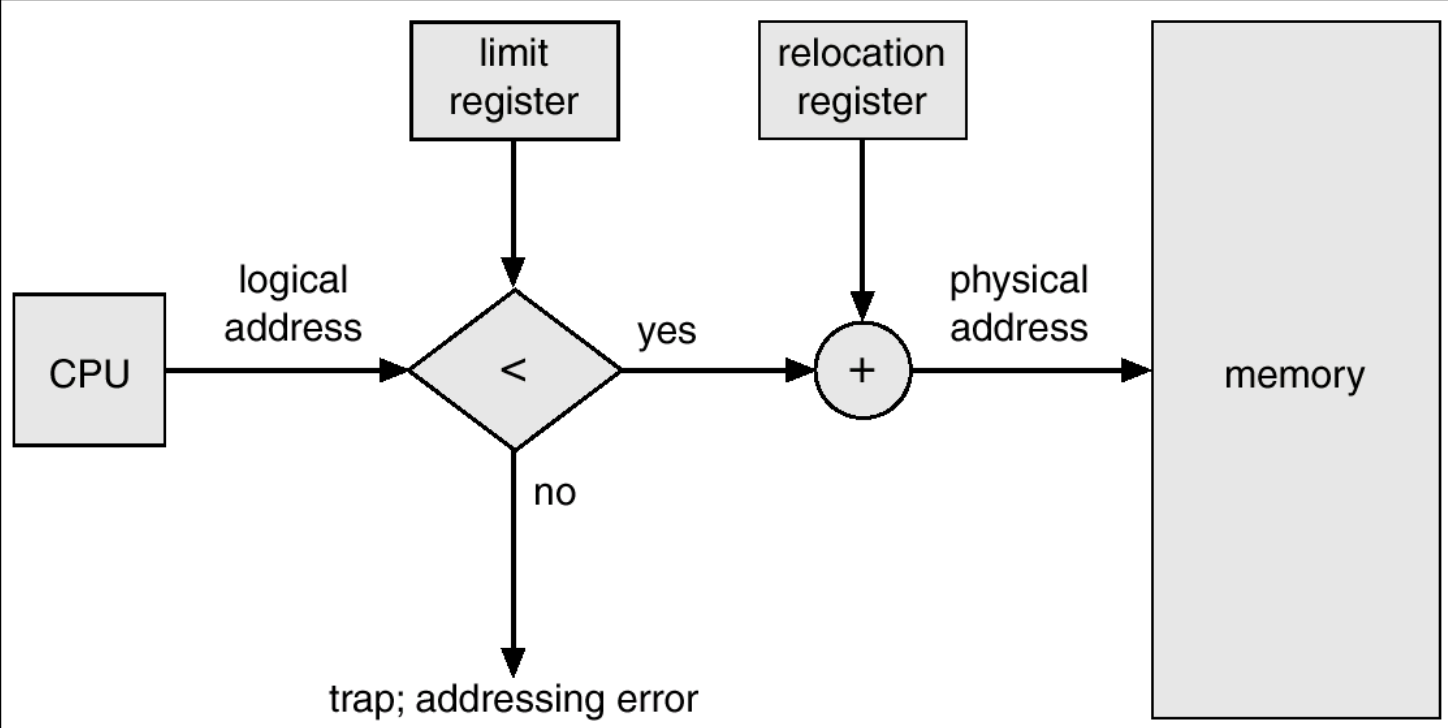
\includegraphics[width=7.5cm]{./photos/base_and_limit.png}
        \captionof*{Fig}{Flow diagram for hardware support}
    \end{center}
\end{aside}
To summarise so far, we know:
\begin{itemize}
    \item We represent free portions of memory with a linked list
    \item We (generally) dynamically parition memory, using first-fit
    \item We 'compact' memory within processes where possible to reduce external fragmentation
    \item We bound the accessible memory for a given process to ensure security
\end{itemize}
How do these above processes and structures interact with concurrency and context switching? If we don't have enough memory, how do we make room for another process?
\subsection{Concurrency, timesharing and swapping}
If our system has to run $n$ processes such that the sum of their required memory is available memory, then we must be able to compromise with the available memory space and 'yield' memory.
\begin{aside}{Timesharing} \\
    There has been this idea of \textit{timesharing} mentioned, where processes in a computer take turns with compute. Similarly, in memory management, we have to consider how processes 'timeshare' memory regions.
\end{aside}
\begin{theory}{Swapping: making space whilst not running} \\
    Swapping involves moving the process \textit{temporarily} out of memory into a \verb|backing store|,and then brough back into memory when required to run.
    \begin{itemize}
        \item Swapping transfers \textit{the entire process}
        \item The backing store is a fast-disk
        \item Prioritisation is generally used to swap out lower-priority process
    \end{itemize}
    Swapping time is proportional to the amount of data in the process, so it is \textit{slow}.
\end{theory}
\subsection{Virtual memory}
Virtual memory aims to be an abstraction of allocating memory space, by serving translated, \verb|virtual| addresses to applications.
\begin{theory}{Paging} \\
    Paging is the idea of partitioning physical memory into small equal sized chunks called \verb|frames|.
    \begin{itemize}
        \item Then each process' address space gets split into the same-sized chunks called \verb|pages|
        \item These pages then represent virtual addresses - which have:
        \begin{enumerate}
            \item A page number
            \item A page offset (as a page can contain main addresses)
        \end{enumerate}
    \end{itemize}
    The operating system then maintains a \textit{page table}, which contains the frame location for each page, and acts as a translation layer.
    \begin{itemize}
        \item[\ding{51}] No external fragmentation - every single page can be used!
        \item[\ding{51}] Minimal internal fragmentation with appropiate sizing
    \end{itemize}
\end{theory}
\begin{aside}{Why should we use paging?} \\ 
    Paging is convenient as memory that is not \textit{necessarily contiguous} can be treated as such by the user application. Therefore, many of our issues that could not be solved (compacting compile time memory) are solved by paging.
\end{aside}
\begin{theory}{Page tables and virtual addresses as indices} \\
    We have pages that translate virtual memory address to physical memory address. With a \verb|32|-bit address, consider that:
    \begin{itemize}
        \item A one-layer table would have $2^{32}$ entries!
        \item So this should motivate some lazy-alloaction...
    \end{itemize}
    But we can't lazy-allocate a single layer table. This motivates a multi-layer table.
    \begin{itemize}
        \item Different portions of the virtual memory address indicate indices into different layers of the page table
        \item The first layer of the page table is \textit{allocated}, and then further layers are \verb|NULL| until utilised.
    \end{itemize}
    \begin{aside}{What do you mean we use the virtual address to index?} \\
        For example, in a \verb|16|-bit address 
        \begin{center}
            \verb|011010;0111000;101|
        \end{center}
        
    \end{aside}
\end{theory}
\begin{aside}{Page table entries} \\
    What sort of information is stored in these page tables? Well a page table should contain
\begin{verbatim}
struct pte {
    int page_frame_number;
    int present;
    int read, write, exec;
    int caching;
    int modified;
    int reference;
}
\end{verbatim}
\begin{itemize}
    \item The page frame number is used to combine with the offset to create the physical address.
    \begin{itemize}
        \item It is the \textit{start} of the address range of the page
    \end{itemize}
    \item \verb|present|: is this page mapped?
    \item \verb|read, write, exec|: protection bits
    \item \verb|caching|: should we bypass the cache? (discussed later)
    \item \verb|modified|: has the page been modified in memory (for writeable)
    \item \verb|reference|: has the page been accessed?
\end{itemize}
\end{aside}
\begin{theory}{Memory management unit (MMU)} \\
    The \verb|MMU| is hardware responsible for translating
    \begin{gather*}
        \text{Virtual address} \implies \text{Physical address}
    \end{gather*}
    The mechanism for this is to use portions of the virtual address to access different layer(s) of the page table, and then use some portion as an \verb|offset|.
    \begin{center}
        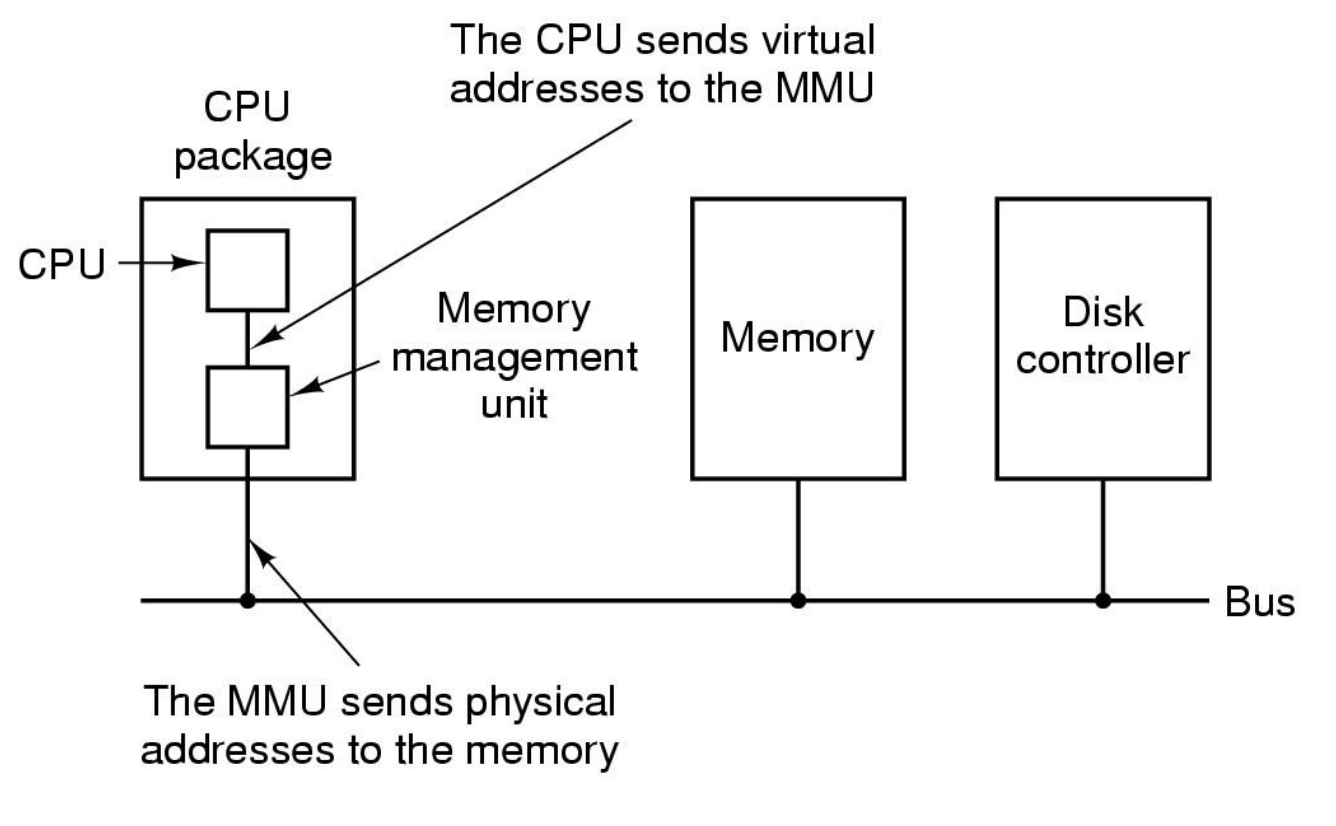
\includegraphics[width=7.5cm]{./photos/tlb.png}
        \captionof*{Fig}{Memory Management Unit (MMU)}
    \end{center}
\end{theory}
\begin{example}{What if a page hasn't been mapped yet? Page faults!}  \\
    Referencing an invalid page will lead to a page fault (an exception) in the operating system. There are broadly two types of pagee faults
    \begin{enumerate}
        \item Illegal address (out of bounds)
        \begin{itemize}
            \item We can just signal or kill the process 
        \end{itemize}
        \item Page not resident (not mapped)
        \begin{itemize}
            \item Find an unused frame, load the page from disk and update the page table
        \end{itemize}
    \end{enumerate}
\end{example}
\begin{aside}{Shared pages} \\
    Much memory is shared between similar processes. It is possible to share pages if it is not self-modifying, and appears at the same address.
\end{aside}
So we now know how modern operating systems divvy up memory to be used by processes - but you may notice some performance issues here.
\begin{itemize}
    \item Virtual memory references are inefficient;
    \item We have to look up the physical memory address to fetch the PTE
    \item And another time, to fetch/store the data
\end{itemize}
How do we improve page tables?
\subsection{Page table improvements and alternatives; inverted, hashed and TLB cache}
We know that page tables grow w.r.t virtual address space - but it would be more desired to have this grow with the size of memory itself to save space.
\begin{aside}{Process IDs in page tables} \\
    In a multiprocessor system, pages are allocated to many different processes. Therefore, process identification (\verb|PID|s) in the form of Address Space Identifiers (\verb|ASID|s) are used to ensure that the accessed process is for the right process.
\end{aside}
\begin{theory}{Inverted Page Table (IPT)} \\
    An array of page numbers indexed by physical frame number which is hashed into an index. Contains information regarding the page.
    \begin{itemize}
        \item Compute the hash of the page number, and extract index
        \item Index into page table, match PID and page number in the entry
        \item If match, use index value as a frame \# for translation
        \item If not match, chain
    \end{itemize}
    IPTs have a few bonuses
    \begin{itemize}
        \item[\ding{51}] IPT grows with the size of RAM, not address space
        \item[\ding{51}] Saves a lot of space, especially as addresses get bigger
    \end{itemize}
\end{theory}
\begin{aside}{IPT improvement: Hashed Page Table (HPT)} \\
    Hash Page Tables (HPT) improve inverted page tables by using a hash function on the virtual address space to access page table entries.
    \begin{itemize}
        \item Page table size is still relative to physical memory size (due to the hash indexing)
    \end{itemize}
\end{aside}
We now consider the improvement of page table accesses. Consider that page tables can lead to \textit{two} physical memory addresses
\begin{itemize}
    \item One to fetch the page table entry
    \item Another to actually \verb|access/write| the data
\end{itemize}
How do we improve on this?
\begin{theory}{Translation Lookaside Buffer (TLB)} \\
    Given a job to translate a virtual address, the \verb|CPU| first looks at the \verb|TLB|
    \begin{itemize}
        \item If a match exists, then there exists a caching of the PFN of this virtual address
        \item Otherwise, theres a TLB miss, and then
        \begin{itemize}
            \item We walk the page table - if it exists, we load this into the TLB
            \item Otherwise, we enter a page fault, and also load this into the TLB
        \end{itemize}
    \end{itemize}
    The TLB is basically an array of frame numbers, which holds recently used page table entry information.
\begin{verbatim}
struct tlb_entry {
    int virtual_address;
    int page_frame_number;
    // protection bits, asid, etc...
}
\end{verbatim}
\end{theory}
The TLB can either be hardware or software loaded - in MIPS R3000, the TLB is software loaded and thus the hardware will generate a TLB miss exception which the software deals with.
\subsection{MIPS R3000 Address Space Layout}
Hardware generally has standardised partitions of the address space that are used for specific components of the operating system.
\begin{theory}{MIPS R3000 Address Space Layout} 
    \begin{center}
        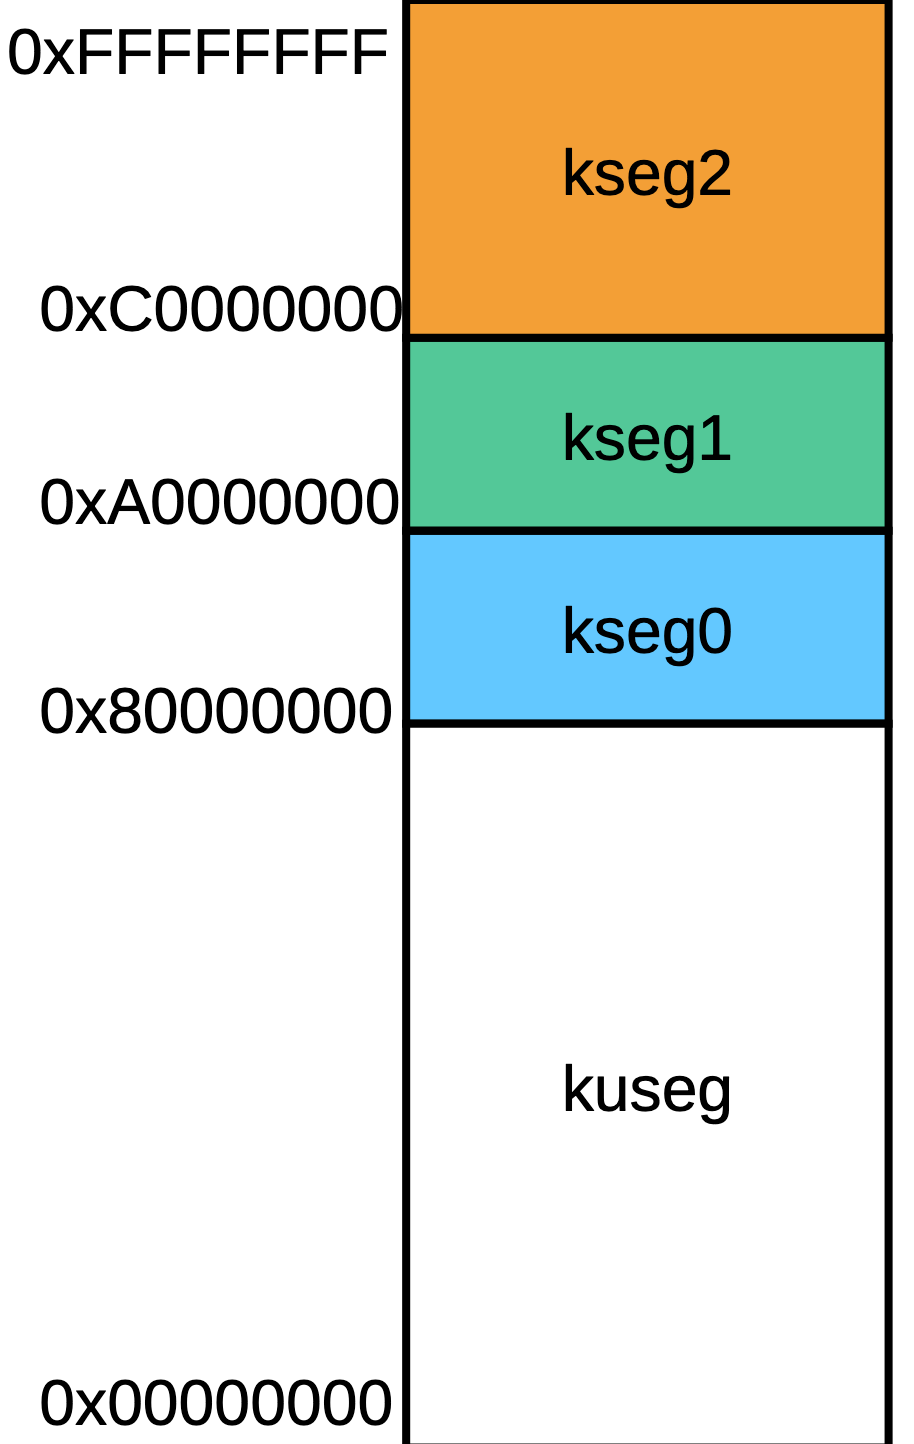
\includegraphics[width=4.5cm]{./photos/r3000_addr.png}
        \captionof*{Fig}{MIPS R3000}
    \end{center}
    \begin{itemize}
        \item \verb|kuseg|: 2 gigabytes, user + kernel, TLB translated
        \item \verb|kseg0|: 512 megabytes, fixed translation window (1:1) to physical, cacheable, kernel code and data
        \item \verb|kseg1|: 512 megabytes, fixed translation window, not cacheable, kernel only, used for devices
        \item \verb|kseg2|: 1 gigabyte, kernel only, TLB translated, dynamic kernel memory
    \end{itemize}
\end{theory}
\subsection{TLB Exception handling in MIPS R3000}
Remember the special exception vectors we were talking about in system calls?
\begin{aside}{Special exception vectors for TLB refill} \\
    For \verb|TLB| misses in \verb|kuseg| (the user allocatable memory region), there is a special exception handler that is optimised for TLB refill.
    \begin{itemize}
        \item Does not need to check the exception type
        \item Does not need to save any registers (only \verb|$k0| and \verb|$k1|)
        \item Does not check if the page table exists
    \end{itemize}
\end{aside}
\begin{example}{Some other virtual memory related exceptions} \\
    These exceptions are handled by the general exception vector
    \begin{itemize}
        \item \verb|TLB Mod|: TLB modify exception, attempt to write to a read-only page
        \item \verb|TLB Load|: Attempt to load from a page with an invalid translation
        \item \verb|TLB Store|: Attempt to store to a page with an invalid translation
    \end{itemize}
\end{example}
\begin{theory}{Amdahl's Law} \\
    Amdahl's Law states that the theoretical speed up of a task is with respects to the part that can be parallelised. Given
    \begin{itemize}
        \item $f$, the fraction of thee task that must remain serial
        \item $(1 - f)$ the fraction of the task that can be parallelised
        \item $N$ the number of processors
    \end{itemize}
    Then the maximum speed up is
    $$ S(N) = \frac{1}{f + \frac{1-f}{N}}$$
\end{theory}
There exists special registers in MIPS R3000 that are for TLB refills.
\begin{theory}{MIPS R3000 TLB Properties} \\
    In \verb|MIPS R3000|, there exists two components in the TLB entry
    \begin{itemize}
        \item \verb|EntryHi| which contains \verb|page #| and ASID
        \item \verb|EntryLo| with contains \verb|frame #| and protection bits
    \end{itemize} 
    There are three special \verb|c0| registers for TLB refills
    \begin{itemize}
        \item \verb|c0_EntryHi|: used to read/write individual TLB entries
        \item \verb|c0_EntryLo|: used to read/write individual TLB entries
        \item \verb|c0_Index|: used as an index to TLB entries
    \end{itemize}
\end{theory}
\begin{aside}{MIPS R3000 TLB Bits}
    \begin{center}
        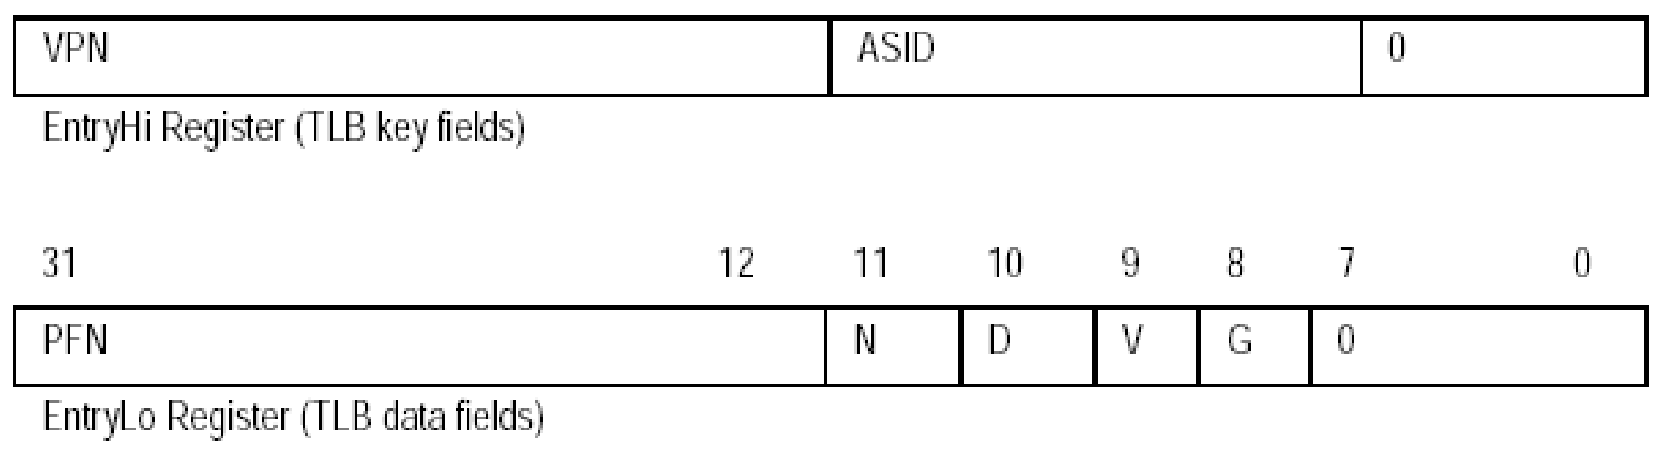
\includegraphics[width=7.75cm]{./photos/r3000_entry.png}
        \captionof*{Fig}{MIPS R3000}
    \end{center}
    \begin{itemize}
        \item N = Not cacheable
        \item D = Dirty
        \item G = Global (ignore ASID)
        \item V = Valid
    \end{itemize}
\end{aside}
\begin{example}{Exam question style: finding TLB matches in a table} \\
    In MIPS R3000, the final 12 bits is the offset. Therefore, the first 20 bits is the VPN given a virtual address.
    \begin{center}
    \begin{tabular}{|c|c|}
    \hline
    \textbf{EntryHi} & \textbf{EntryLo} \\
    \hline
    \verb|0x00028200| & \verb|0x0063f400| \\
    \hline
    \end{tabular}
    \end{center}
    Given that the current EntryHi is \verb|0x00000200|, we have that the ASID is \verb|0x200|, therefore we should only consider EntryHi's that end with \verb|0x200|.
    \begin{itemize}
        \item Consider we look for \verb|a = 0x00028123|
        \item The VPN is \verb|a >> 12|, therefore \verb|0x00028|
        \item This matches with our table entry, and the ASID matches too.
        \item Check the permission bits of EntryLo.
        \item Valid bit is set to 0, therefore INVALID mapping.
        \item Otherwise, physical address would be \verb|0x0063f123|
    \end{itemize}
    \vspace{0.5cm}
    \begin{center}
    \begin{tabular}{|c|c|}
    \hline
    \textbf{EntryHi} & \textbf{EntryLo} \\
    \hline
    \verb|0x0005b200| & \verb|0x002af200| \\
    \hline
    \end{tabular}
    \end{center}
    \begin{itemize}
        \item Consider we look for \verb|a = 0x0005b888|.
        \item The VPN matches, \verb|0x0005b|
        \item The ASID matches (if it doesn't check for global)
        \item Now consider the low bits.
        \item We have \verb|0x200| = \verb|001100000000|
        \item Dirty bit is 0, so read only, and a valid mapping.
    \end{itemize}
\end{example}
\begin{example}{MIPS R3000 TLB management instructions} \\
    \begin{itemize}
        \item \verb|TLBR|: reads in to EntryHi and EntryLo w.r.t index register
        \item \verb|TLBP|: reads in EntryLo given an EntryHi
        \item \verb|TLBWR|: writes EntryHi and EntryLo to a pseudo-random position
        \item \verb|TLBWI|: writes EntryHi and EntryLo to aa location pointed to by the index register
    \end{itemize}
\end{example}
\subsection{Paging performance considerations}
We now consider different performance considerations of paging, such as
\begin{itemize}
    \item Should we load pages on demand?
    \item Should we predictively load pages for processes?
\end{itemize}
\begin{theory}{Principle of Locality: things close together are used together}
    \begin{center}
        \textit{Programs tend to reuse data and instructions they have used recently.}
    \end{center}
    You can then motivate that we can exploity this 'locality' of references. We could reasonably predict that given some instructions and data, we have some idea of what data/instructions will be needed.
    \begin{enumerate}
        \item \textbf{Temporal} locality: recently accessed items are likely to be accessed in the near future (caching)
        \item \textbf{Spatial} locality: items whose addresses are near one another tend to be referenced close together in time
    \end{enumerate}
\end{theory}
\begin{theory}{Working set: what does a program need in a given time period?}
    \begin{center}
        \textit{The pages required by an application in some time window $\Delta$ is called it's memory working set}
    \end{center}
    Note that it is defined in \textit{pages}. Therefore, the \textit{working set} $\approx$ program's locality. If $\Delta^*$ is an estimator for $\Delta$, the true locality window
    \begin{itemize}
        \item As $\Delta^* \ll \Delta$, the time window does not encompass the entire locality
        \item As $\Delta^* \gg \Delta$, the time window compasses severl localities
    \end{itemize}
\end{theory}
\begin{aside}{So what is a good $\Delta$?} \\
    A good $\Delta$ approximates what is required for execution without having too much irrelevant information.
    \begin{itemize}
        \item The working set tends to change gradually
    \end{itemize}
\end{aside}
This motivates one method of loading pages - \verb|demand| paging.
\begin{aside}{Demand paging: get what you need} \\
    In demand paging, we reload non-resident pages on demand (when we require them). With the principle of locality, it should be true that we rarely access non-resident pages.
\end{aside}
But what occurs when we have a lot of processes in memory that all demand more and more pages? Eventually, with enough multiprogramming, every process will keep requesting pages but never have the \textbf{resident set} required.
\begin{aside}{What is the required resident set?} \\
    The \verb|resident set| refers to the pages that are loaded in the page table/physical memory, and have valid mappings.
    \newline \\
    A process' \textit{required} resident set is the pages it requires to execute it's current task.
\end{aside}
\begin{theory}{Thrashing: too many requests!} \\
    As \# of processes $\uparrow$, the amount of memory for each process $\downarrow$.
    \begin{itemize}
        \item Therefore the available resident set for each process decreases
        \item With this, the amount of demand paging increases
        \item But since every process demands more pages, processes don't get there required resident set
    \end{itemize}
    So while multiprogramming $\uparrow$ CPU utilisation, at some point processes do not have the required resident set and cannot run.
    \begin{center}
        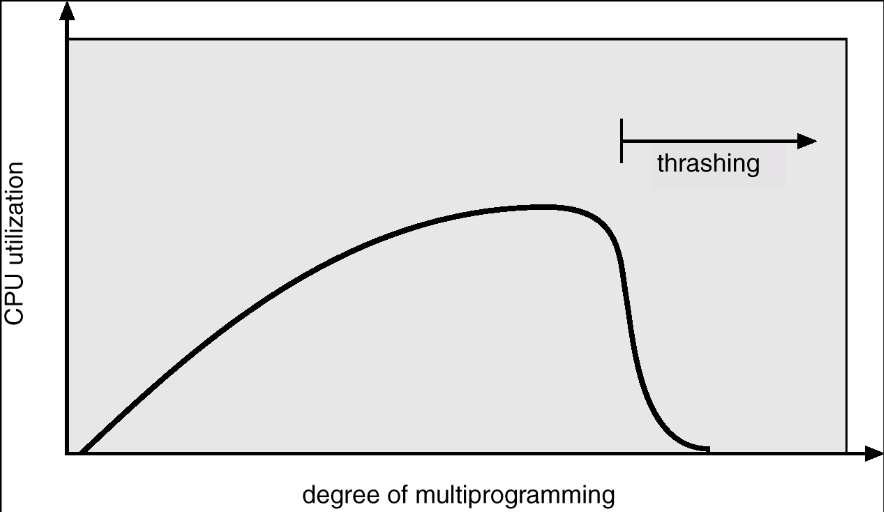
\includegraphics[width=7.5cm]{./photos/thrashing.png}
        \captionof*{Fig}{Thrashing occurs beyond a certain point}
    \end{center}
\end{theory}
To recover from thrashing, we can simply suspend a few processes to provide more memory.
\begin{example}{A demonstrative example of locality: what's faster?} \\ 
    We previously talked about how things that are close together (have locality) are often accessed together. Consider the below code snippet.
    \begin{verbatim}
int array[10000][10000];
int i, j;
for (int i = 0; i < 10000; ++i) {
    for (int j = 0; j < 10000; ++j) {
        array[i][j] = 0;
        array[j][i] = 0;
        // what's faster?
    }
}\end{verbatim}
    In this case, accessing the arrays in order \verb|[i][j]| is faster, as they are more local (2D arrays are an array of arrays).
    \begin{itemize}
        \item Row wise access has more spatial locality, and is more cache friendly
        \item Column-wise access skips between many memory addresses
    \end{itemize}
\end{example}
\subsection{Virtual memory management policies}
There are a few considerations for virtual memory that you may have noticed so far.
\begin{itemize}
    \item Page table format; multi-level? inverted? hashed?
    \item Page size
    \item Fetch policy
    \item Replacement policy
    \item Resident set size
    \item Page cleaning policy
\end{itemize}
\begin{aside}{Page size: how much memory should pages hold?} \\ 
    As page size $\uparrow$
    \begin{itemize}
        \item[\ding{51}] Decreases number of pages
        \item[\ding{51}] Increases TLB coverage (more data per TLB entry) 
        \item[\ding{51}] Increassing swapping I/O throughput
        \item[\ding{55}] Increases internal fragmentation
        \item[\ding{55}] Increases page fault latency (more data to read from disk)
    \end{itemize}
\end{aside}
\begin{aside}{Fetch policy: how should we fetch pages?} \\
    We have two options
    \begin{enumerate}
        \item Demand paging
        \begin{itemize}
            \item Lots of page faults when a process first starts
            \item But we make no assumptions about the processes
        \end{itemize}
        \item Pre-paging
        \begin{itemize}
            \item Pre-paging brings in pages in anticipation of a program's working set
            \item Wastes \verb|I/O| if pages are not used
        \end{itemize}
    \end{enumerate}
\end{aside}
\begin{aside}{Replacement policy: when pages are full, which one should we evict?} \\
    When the page table is full, which page should be chosen to vacate a frame?
    \begin{itemize}
        \item Page removed should be the page least likely to be referenced in the near future
        \item There are some frames that are \textbf{locked} - important to kernel operation for e.g
        \item The frame table has a \verb|pinned| bit/flag to keep track of this
    \end{itemize}
    Consider some replacement policies
    \begin{example}{First-in, first-out (FIFO)} \\
        Just remove the oldest page. The age of a page is not necessarily related to it's usage in the near future however
    \end{example}
    \begin{example}{Least Recently Used (LRU)} \\ 
        Choose the leaast recently used page. Assumes if a page has not been references for a long time, it is unlikely to be referenced in the near future
        \begin{itemize}
            \item Is true under the principle of locality
            \item A time stamp is required for each page (but is proxied)
        \end{itemize}
    \end{example}
\end{aside}
What are some proxies for least recently used?
\begin{example}{\texttt{LRU} proxy: clock page replacement} \\
    In clock page replacement, the frames are ordered in a circular fashion and a 'clock hand' (the CPU clock) points to one frame at a time
    \begin{itemize}
        \item Have a \verb|reference| bit in the frame table
        \item Set to \verb|1| when page is used
        \item As you scan for a replacement, if
        \begin{enumerate}
            \item If $\verb|R = 0|$ evict this page
            \item If $\verb|R = 1|$, set to $\verb|0|$
        \end{enumerate}
    \end{itemize}
    Since recently used pages ($\verb|R = 1|$) get a 'second chance', it is also called second chance replacement.
\end{example}
\begin{aside}{Resident set size: how many frames should each process have?}
    \begin{itemize}
        \item Fixed allocation
        \begin{itemize}
            \item Gives a process a fixed number of pages
            \item High utilisation is an issue, requirement for different processes has high skew
        \end{itemize}
        \item Variable allocation
        \begin{itemize}
            \item Number of pages allocated to a process varies over the lifetime of the process
        \end{itemize}
    \end{itemize}
    We differ variable allocation by the scope of 'variability'
    \begin{example}{Global scope} \\
        The OS keeps a global list of free frames, and allocates frames to process on a need basis.
        \begin{itemize}
            \item[\ding{51}] Automatic balancing across system
            \item[\ding{55}] Does not provide guarantees for high-priority processes
        \end{itemize}
    \end{example}
    \begin{example}{Local scope} \\
        The OS allocates page frames based on a few criterion
        \begin{itemize}
            \item Application type
            \item Program request
            \item Other criteria like priority, etc
        \end{itemize}
    \end{example}
\end{aside}
\begin{aside}{Cleaning policy: how do we deal with dirty (written) pages?} \\
    Pages can be written to and modified in memory. These changes need to be written to disk eventually. There are two main approaches:
    \begin{enumerate}
        \item Demand cleaning
        \begin{itemize}
            \item Write out page only when it is selected for replacement
            \item However this means the replaced page has high latency until ready (write times are long)
        \end{itemize}
        \item Pre-cleaning
        \begin{itemize}
            \item Pages are written out in batches in the background
            \item Increases likelihood of replacing clean frames
            \item Overlap \verb|I/O| with current CPU activity
        \end{itemize}
    \end{enumerate}
    It is clear that it is faster to replace clean pages as no writes occur, so we want to replace clean pages where possible.
\end{aside}
\section{Multiprocessor systems and their implications} 
In modern compute, we have seen an exponential growth and then tapering of CPU clock-rate, but a constant exponential growth of \textit{core count}.
\newline \\
As the number of \textit{CPUs}/\textit{cores} grow, the way we handle concurrent memory accesses for multiple processors becomes an issue.
\begin{theory}{Bus-based uniform memory access multiprocessors} \\
    Bus-based \verb|UMA| multiprocessors are structured such that each CPU/core share a single memory bus to access memory.
    \begin{itemize}
        \item Bus controller/mechanism resolves parallel access
        \item Access to all memory occurs at roughly the same speed for all processors
    \end{itemize}
    \begin{center}
        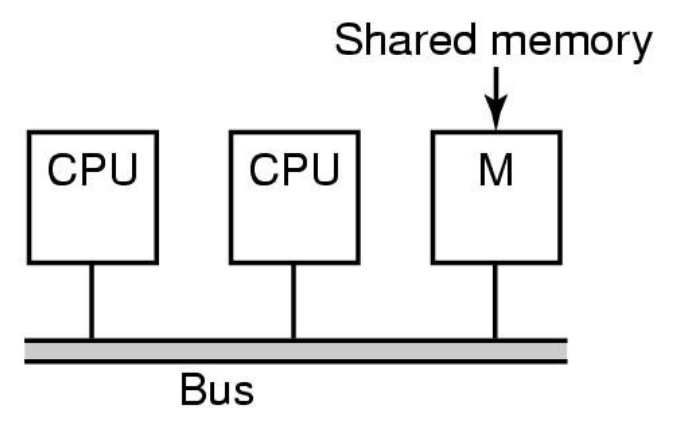
\includegraphics[width=6.5cm]{./photos/uma.png}
        \captionof*{Fig}{Bus-based multiprocessors}
    \end{center}
    There are clearly considerations to be made with sharing a bus and memory - which we will consider next.
\end{theory}
\begin{aside}{Consideration 1: Adding caches, and cache consistency} \\ 
    Each CPU has it's own cache to increase memory fetch performance, as constantly using the \verb|bus| would grow to be unscalable.
    \newline \\ 
    But how do we deal with consistency of cached memory across CPUs?
    \begin{itemize}
        \item Generally handled by hardware
        \item Writes to one cache propagates to \textit{or} invalidates entries on other caches
        \item But cache transactions consume bus bandwidth
    \end{itemize}
\end{aside}
\begin{aside}{Consideration 2: How do we run an OS for multiple processors?} \\
    There are two approaches to running an OS for multiple processors
    \begin{enumerate}
        \item Per-CPU OS
        \begin{itemize}
            \item[\ding{51}] Simpler to implement
            \item[\ding{51}] Scalable, as there is no shared serial sections
            \item[\ding{55}] Each processor has it's own scheduling queue
            \item[\ding{55}] Each processor has it's own memory partition
        \end{itemize}
        \item Shared OS (Symmetric Multiprocessors)
        \begin{itemize}
            \item[\ding{51}] Load and resource balancing between processors
            \item[\ding{55}] Concurrency in the kernel, so synchronisation available
        \end{itemize}
    \end{enumerate}
\end{aside}
\begin{example}{Why should we share the kernel? What advantages/disadvantages does this have?} \\
    Sharing the kernel between multiprocessors has the following implications
    \begin{itemize}
        \item[\ding{51}] Get global scheduling, which ensures that CPU's are treated equally
        \item[\ding{51}] Automatic load balancing
        \item[\ding{55}] Treating equally not always great, some CPUs have hot caches
        \item[\ding{55}] Per-CPU OS gives more control, by avoiding contention, by is more complex 
    \end{itemize}
\end{example}
\begin{example}{Symmetric multiprocessors: synchronising the kernel}
    \begin{center}
        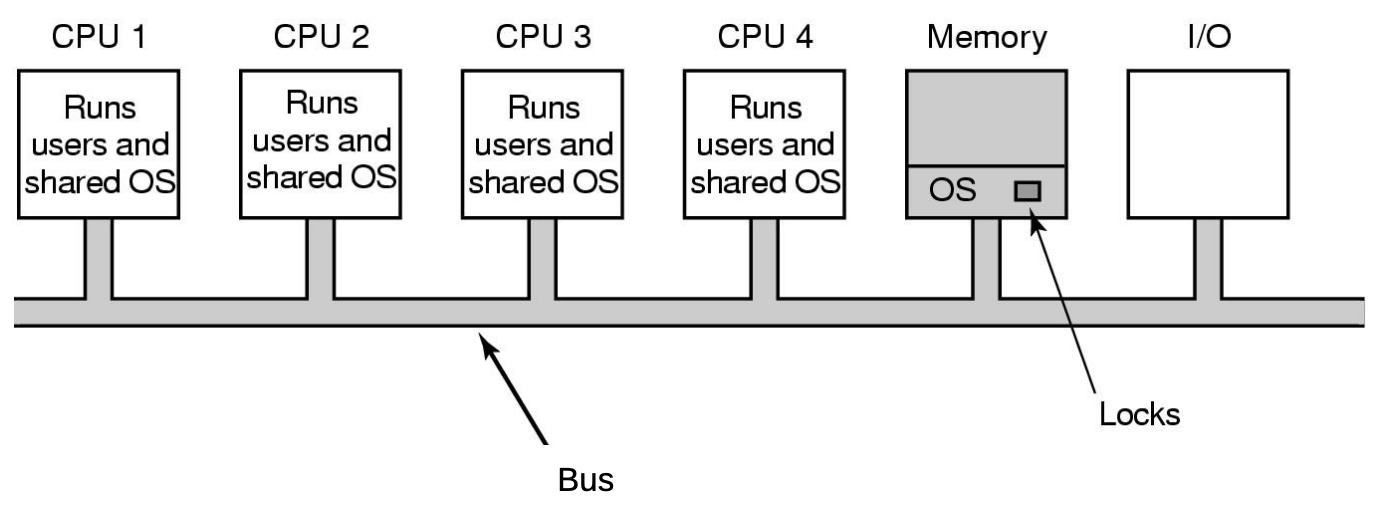
\includegraphics[width=7.75cm]{./photos/smp.png}
        \captionof*{Fig}{Symmetric multiprocessor}
    \end{center}
    There are a few approaches to deal with synchronisation in the OS
    \begin{enumerate}
        \item A big lock around the entire kernel
        \begin{itemize}
            \item Obviously this will be a large bottle neck, as this is essentially a single-threaded kernel
        \end{itemize}
        \item Mutex independent parts of the kernel
        \begin{itemize}
            \item Requires complex lock ordering and analysis
            \item But far more efficient and allows parallel computation
        \end{itemize}
    \end{enumerate}
\end{example}
Now we know how to synchronise the kernel, how do we synchronise variables?
\begin{example}{Why can't we preempt spinlocking processes?} \\
    Consider a process $P_1$ that is spin-locking for the access of some variable $v$.
    \begin{itemize}
        \item Given preemption is allowed, the scheduler will attempt to block
        \item But preemption of lock holders extends the time of the spin-locks
        \item Therefore we waste more time in context switching
    \end{itemize}
    
\end{example}
\begin{theory}{Multiprocessor synchronisation: read, test \textit{then} set} \\
    In \verb|test-and-set|, we spinlock at the test until the variable is ready to be taken. Why is this not plausible for multiprocessor systems?
    \begin{itemize}
        \item Read the above example for reasoning
        \item So we have to block all other CPUs from accessing the bus during \verb|TSL|
    \end{itemize}
    We instead \textbf{read, then test and set} on a multi processor system.
    \begin{enumerate}
        \item Read the lock variable, if it is not taken
        \item Attempt to \verb|test-and-set|
        \item If not successful, continue spin-locking on the read
    \end{enumerate}
    \begin{verbatim}
start:
    // spin on read
    while (lock == 1)
        ;
    
    // try taking
    r = TSL(lock);
    
    // got taken already
    // re-spin
    if (r == 1)
        goto start;\end{verbatim}
    This means that only the processor is spinlocking instead of the entire machine being blocked.
\end{theory}
\begin{aside}{Hold on; why don't we just block like a uniprocessor system?} \\
    In our original discussion about test-and-set, we said that blocking a waiting thread was more efficient than spinlocking, so why don't we do this?
    \begin{itemize}
        \item Switching to another process is \textit{costly}
        \item Spinning wastes CPU time \textit{directly} - but switching to another process is \textit{atomic}
        \item If a lock becomes available mid-way through a switch, then we must switch back 
        \item And this wastes time during the switch
    \end{itemize}
    As a rule of thumb:
    \begin{center}
        If the lock will be held for longer than $2\times$ the switching overhead, then it's more efficient to block.
    \end{center}
\end{aside}
\begin{example}{Blending blocking and spinning with a hybrid lock} \\
    An easy way to blend the positives of switching and spinning is to have a hybrid lock that
    \begin{itemize}
        \item Attempts to take the lock with test-and-set
        \item If it fails, spins with read then test-and-set for $\approx$ 1000 cycles
        \item Then switches threads
    \end{itemize}
\end{example}
\end{document}